\subsection{Tipologia di utenti}
Prima di procedere con l’elenco degli \glossaryItem{Use Case}, vengono specificati i tipi di utenti che possono interagire con l'\glossaryItem{Applicazione}.
\begin{figure}[h!]
\centering
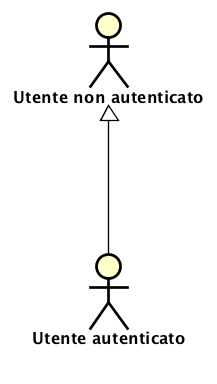
\includegraphics[scale=0.5]{../../Casi D'uso/TipologiaUtenti.png}
\caption{Gerarchia degli utenti}
 \end{figure}

 Descrizione degli utenti:

 \begin{itemize}
 \item \textbf{Utente non autenticato}: è un \glossaryItem{Utente} che posside un \glossaryItem{Account}, ma deve ancora effettuare l'autenticazione; oppure un \glossaryItem{Utente} che intende effettuare la registrazione per poi autenticarsi.
 \item \textbf{Utente autenticato}: è un \glossaryItem{Utente} che ha effettuato l'autenticazione e che può utilizzare le funzionalità dell'\glossaryItem{Applicazione}.
 \end{itemize}

\subsection{Notazione Use Case}
L'analisi del \glossaryItem{Capitolato}, l'incontro con Zucchetti S.r.l. e la discussione tra gli \emph{Analisti} ha portato alla definizione dei seguenti casi d'uso.\\
Ogni caso d’uso presente ha un \glossaryItem{Codice} univoco gerarchico, nella forma:
\[UC[Codice del padre].[Codice progressivo di livello]\]
Il \glossaryItem{Codice} progressivo può includere diversi livelli di gerarchia separati da un punto.

\newpage
\subsection{UC0 - Visione Generale}
\label{ssec:UC0}
\begin{figure}[h!]
\centering
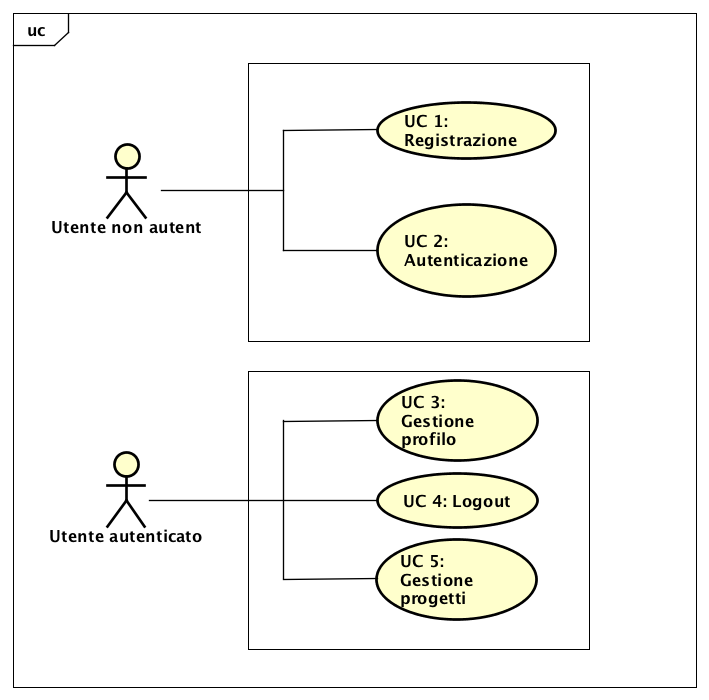
\includegraphics[scale=0.5]{../../Casi D'uso/Generale.png}
\caption{Caso d'uso UC0}
 \end{figure}
\begin{itemize}
\item \textbf{Attori}: \glossaryItem{Utente} non autenticato e \glossaryItem{Utente} autenticato;
\item \textbf{Descrizione}: Vengono visualizzate in generale le vari funzionalità che l'\glossaryItem{Applicazione} permette ai vari utenti di svolgere;
\item \textbf{Precondizione}: L'\glossaryItem{Applicazione} predispone l'interazione con un attore, facendolo accedere alle diverse funzionalità proposte;
\item \textbf{Postcondizione}: Dopo l'interazione avvenuta con un attore, l'\glossaryItem{Applicazione} si troverà in un nuovo stato pronto ad interagire con un nuovo attore;
\item \textbf{Scenario principale}: \begin{enumerate}\item Registrazione (UC1);\item Autenticazione (UC2);\item Gestione profilo(UC3);\item Logout (UC4);\item Gestione progetti (UC5);\item Tool \glossaryItem{Designer} (UC6);
 \end{enumerate}
\end{itemize}

\subsection{UC1 - Registrazione}
\label{ssec:UC1}
\begin{figure}[h!]
\centering
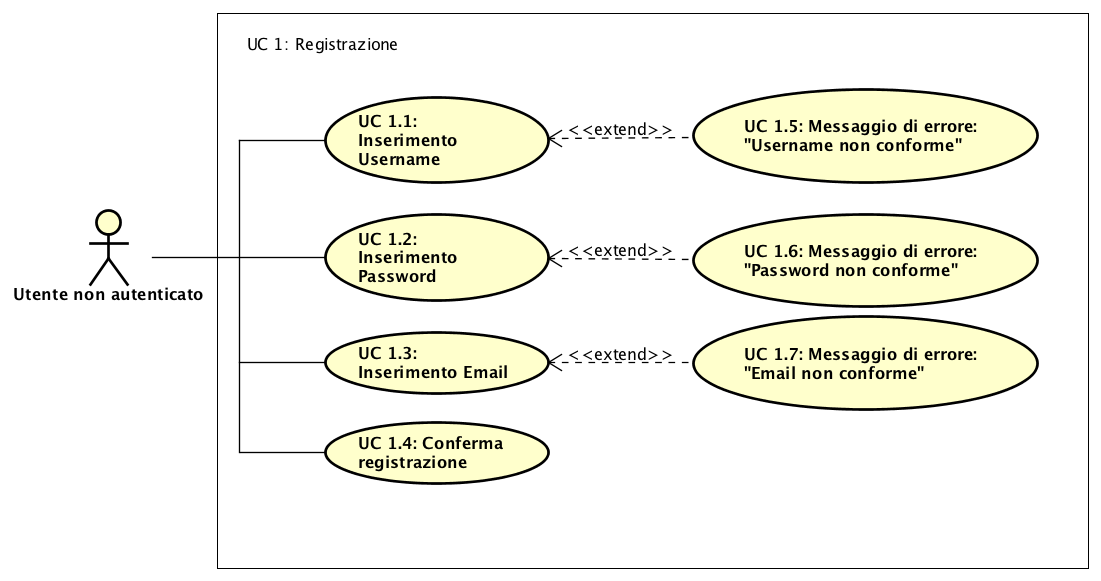
\includegraphics[scale=0.5]{../../Casi D'uso/UC1.png}
\caption{Caso d'uso UC1}
 \end{figure}
\begin{itemize}
\item \textbf{Attori}: \glossaryItem{Utente} non autenticato;
\item \textbf{Descrizione}: L'attore desidera effettuare l'operazione di registrazione. Vengono richiesti dall'\glossaryItem{Applicazione} un \glossaryItem{Username}, univoco e conforme alle richieste, una password conforme alle richieste e una mail che rispetti il \glossaryItem{Pattern} predefinito;
\item \textbf{Precondizione}: L'\glossaryItem{Applicazione} predispone la possibilità di registrazione;
\item \textbf{Postcondizione}: L'\glossaryItem{Applicazione} ha creato un nuovo \glossaryItem{Account} \glossaryItem{Utente};
\item \textbf{Scenario principale}: \begin{enumerate}\item Inserimento \glossaryItem{Username} (UC1.1);\item Inserimento Password (UC1.2);\item Inserimento Email (UC1.3);\item Conferma registrazione (UC1.4).
\end{enumerate}
\item \textbf{Scenari alternativi}:
	\begin{itemize}
	\item Messaggio di errore: "\glossaryItem{Username} non conforme" (UC1.5);\item Messaggio di errore: "Password non conforme" (UC1.6);\item Messaggio di errore: "Email non conforme" (UC1.7).
	\end{itemize}
\end{itemize}
\subsection{UC1.1 - Inserimento Username}
\label{ssec:UC1.1}
\begin{itemize}
\item \textbf{Attori}: \glossaryItem{Utente} non autenticato;
\item \textbf{Descrizione}: L’attore inserisce l'\glossaryItem{Username}: deve essere univoco all'interno dell'\glossaryItem{Applicazione} e può essere alfanumerico;
\item \textbf{Precondizione}: L'\glossaryItem{Applicazione} è pronta e l'attore intende autenticarsi;
\item \textbf{Postcondizione}: L'\glossaryItem{Applicazione} ha l’informazione relativa all'email inserita dall’attore;
\item \textbf{Scenario principale}: L'attore inserisce l'username.
\end{itemize}
\subsection{UC1.2 - Inserimento Password}
\label{ssec:UC1.2}
\begin{itemize}
\item \textbf{Attori}: \glossaryItem{Utente} non autenticato;
\item \textbf{Descrizione}: L’attore inserisce la password: deve essere di tipo alfanumerico e può contenere caratteri di punteggiatura e di almeno 8 caratteri;
\item \textbf{Precondizione}: L'attore intende effettuare la registrazione inserendo la password;
\item \textbf{Postcondizione}: L'attore ha inserito una password conforme alle richieste dell'\glossaryItem{Applicazione};
\item \textbf{Scenario principale}: L'attore inserisce la password.
\end{itemize}
\subsection{UC1.3 - Inserimento Email}
\label{ssec:UC1.3}
\begin{itemize}
\item \textbf{Attori}: \glossaryItem{Utente} non autenticato.
\item \textbf{Descrizione}: L’attore inserisce l'email per effettuare la registrazione;
\item \textbf{Precondizione}: L'attore ha selezionato l'opzione di registrazione e non ha ancora inserito un email;
\item \textbf{Postcondizione}: L'\glossaryItem{Applicazione} ha l’informazione relativa alla password inserita dall’\glossaryItem{Utente};
\item \textbf{Scenario principale}: L'attore inserisce l'email.
\end{itemize}
\newpage
\subsection{UC1.4 - Conferma registrazione}
\label{ssec:UC1.4}
\begin{itemize}
\item \textbf{Attori}: \glossaryItem{Utente} non autenticato;
\item \textbf{Descrizione}: Dopo che un attore ha effettuato correttamente una registrazione, ne viene informato;
\item \textbf{Precondizione}: L'attore ha scelto di effettuare l'operazione di registrazione;
\item \textbf{Postcondizione}: L'attore ha ricevuto un messaggio di conferma dell'avvenuta registrazione;
\item \textbf{Scenario principale}: L' attore viene avvisato dell'avvenuta registrazione.
\end{itemize}
\subsection{UC1.5 - Messaggio di errore: "\glossaryItem{Username} non conforme"}
\label{ssec:UC1.5}
\begin{itemize}
\item \textbf{Attori}: \glossaryItem{Utente} non autenticato;
\item \textbf{Descrizione}: L'attore può inserire un \glossaryItem{Username} non conforme e gli viene quindi comunicato l'errore. Le non conformità sono date dall'inserimento di un username già presente a database, o dalla presenza di caratteri non alfanumerici;
\item \textbf{Precondizione}: L'\glossaryItem{Applicazione} è pronta e l'\glossaryItem{Utente} intende registrarsi;
\item \textbf{Postcondizione}: L'attore ha inserito un \glossaryItem{Username} non conforme e ha ricevuto la comunicazione dell'errore;
\item \textbf{Scenario principale}: L'attore viene avvisato che l'username non è conforme.
\end{itemize}
\subsection{UC1.6 - Messaggio di errore: "Password non conforme"}
\label{ssec:UC1.6}
\begin{itemize}
\item \textbf{Attori}: \glossaryItem{Utente} non autenticato;
\item \textbf{Descrizione}: L'attore può inserire una password non conforme e gli viene quindi comunicato l'errore. Le non conformità sono date dall'inserimento di una password inferiore agli 8 caratteri, o dalla presenza di caratteri non alfanumerici o di punteggiatura;
\item \textbf{Precondizione}: L'\glossaryItem{Applicazione} è pronta e l'\glossaryItem{Utente} intende registrarsi;
\item \textbf{Postcondizione}: L'attore ha inserito una password non conforme e ha ricevuto la comunicazione dell'errore;
\item \textbf{Scenario principale}: L'attore viene avvisato che la password non è conforme.
\end{itemize}
\subsection{UC1.7 - Messaggio di errore: "Email non conforme"}
\label{ssec:UC1.7}
\begin{itemize}
\item \textbf{Attori}: \glossaryItem{Utente} non autenticato;
\item \textbf{Descrizione}: L'attore può inserire un'email con una sintassi non valida e gli viene quindi comunicato l'errore. La non conformità è data dalla presenza di una Email diversa dal formato: "\emph{nomeutente@dominio}";
\item \textbf{Precondizione}: L'\glossaryItem{Applicazione} è pronto e l'\glossaryItem{Utente} intende registrarsi;
\item \textbf{Postcondizione}: L'attore ha inserito un'email non conforme e ha ricevuto la comunicazione dell'errore;
\item \textbf{Scenario principale}: L'attore viene avvisato che l'email non è conforme.
\end{itemize}
\newpage
\subsection{UC2 - Autenticazione}
\label{ssec:UC2}
\begin{figure}[h!]
\centering
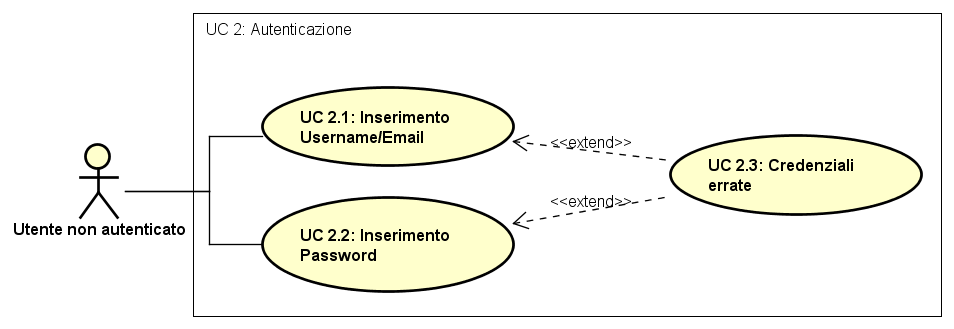
\includegraphics[scale=0.5]{../../Casi D'uso/UC2.png}
\caption{Caso d'uso UC2}
 \end{figure}
\begin{itemize}
\item \textbf{Attori}: \glossaryItem{Utente} non autenticato;
\item \textbf{Descrizione}: L'attore che già in possesso delle credenziali per accedere all'\glossaryItem{Applicazione}, potrà effettuare l'operazione di autenticazione inserendo l'email/\glossaryItem{Username} e la password. Nel caso l’attore abbia perso la password o se la sia dimenticata, l'\glossaryItem{Applicazione} fornisce la possibilità di averne una temporanea per poi resettarla;
\item \textbf{Precondizione}: L'attore decide di autenticarsi e l'\glossaryItem{Applicazione} richiede l'inserimento dei dati necessari per l'autenticazione;
\item \textbf{Postcondizione}: L'attore ha avuto accesso alle funzionalità del l'\glossaryItem{Applicazione}, in caso l'autenticazione sia avvenuta con successo, altrimenti viene visualizzato un messaggio d'errore.
\item \textbf{Scenario principale}: \begin{enumerate}\item Inserimento \glossaryItem{Username}/Email (UC2.1);\item Inserimento Password (UC2.2);\item Password dimenticata (UC2.3);  \end{enumerate}

\item \textbf{Scenari alternativi}: \begin{enumerate}
\item Credenziali errate (UC2.4);\item Invio password per email (UC2.5). \end{enumerate}

\end{itemize}
\subsection{UC2.1 - Inserimento \glossaryItem{Username}/Email}
\label{ssec:UC2.1}
\begin{itemize}
\item \textbf{Attori}: \glossaryItem{Utente} non autenticato;
\item \textbf{Descrizione}: Durante la fase di autenticazione viene richiesto all'attore il proprio \glossaryItem{Username} oppure la propria email;
\item \textbf{Precondizione}: L'\glossaryItem{Applicazione} è pronta e l'attore intende autenticarsi;
\item \textbf{Postcondizione}: L'\glossaryItem{Applicazione} ha l’informazione relativa all'email/\glossaryItem{Username} inserita dall’attore;
\item \textbf{Scenario principale}: L'attore inserisce l'username oppure l'email.
\end{itemize}
\subsection{UC2.2 - Inserimento Password}
\label{ssec:UC2.2}
\begin{itemize}
\item \textbf{Attori}: \glossaryItem{Utente} non autenticato;
\item \textbf{Descrizione}: Durante la fase di autenticazione viene richiesta all'attore la propria password;
\item \textbf{Precondizione}: L'\glossaryItem{Applicazione} è pronta e l'attore intende autenticarsi;
\item \textbf{Postcondizione}: L'\glossaryItem{Applicazione} ha l’informazione relativa alla password inserita dall’attore;
\item \textbf{Scenario principale}: L'attore inserisce la password.
\end{itemize}
\subsection{UC2.3 - Password dimenticata}
\label{ssec:UC2.3}
\begin{itemize}
\item \textbf{Attori}: \glossaryItem{Utente} non autenticato;
\item \textbf{Descrizione}: L'attore ha smarrito la password e l'\glossaryItem{Applicazione} può fornirgliene una temporanea;
\item \textbf{Precondizione}: L'attore possiede un \glossaryItem{Account} all'interno dell'\glossaryItem{Applicazione}, ma non è più in possesso della password;
\item \textbf{Postcondizione}: L'attore ha ricevuto una email contenente la nuova password temporanea;
\item \textbf{Scenario principale}: Viene fornita all'attore una password temporanea.
\end{itemize}
\subsection{UC2.4 - Credenziali errate}
\label{ssec:UC2.4}
\begin{itemize}
\item \textbf{Attori}: \glossaryItem{Utente} non autenticato;
\item \textbf{Descrizione}: L’attore visualizza un messaggio di errore dato dall’inserimento di credenziali errate;
\item \textbf{Precondizione}: L'\glossaryItem{Applicazione} ha verificato le credenziali inserite dall’attore;
\item \textbf{Postcondizione}: L'\glossaryItem{Applicazione} predispone la visualizzazione di un messaggio di errore;
\item \textbf{Scenario principale}: L'attore viene avvisato che le credenziali sono errate.
\end{itemize}
\subsection{UC2.5 - Invio password per email}
\label{ssec:UC2.5}
\begin{itemize}
\item \textbf{Attori}: \glossaryItem{Utente} non autenticato;
\item \textbf{Descrizione}: Viene inviata una password temporanea all'attore per permettergli di accedere all'\glossaryItem{Applicazione};
\item \textbf{Precondizione}: L'attore richiede una password temporanea;
\item \textbf{Postcondizione}: L'\glossaryItem{Applicazione} ha inviato all'attore una mail contenente la password temporanea;
\item \textbf{Scenario principale}: Viene inviata via mail una password temporanea.
\end{itemize}
\newpage
\subsection{UC3 - Gestione Profilo}
\label{ssec:UC3}
\begin{figure}[h!]
\centering
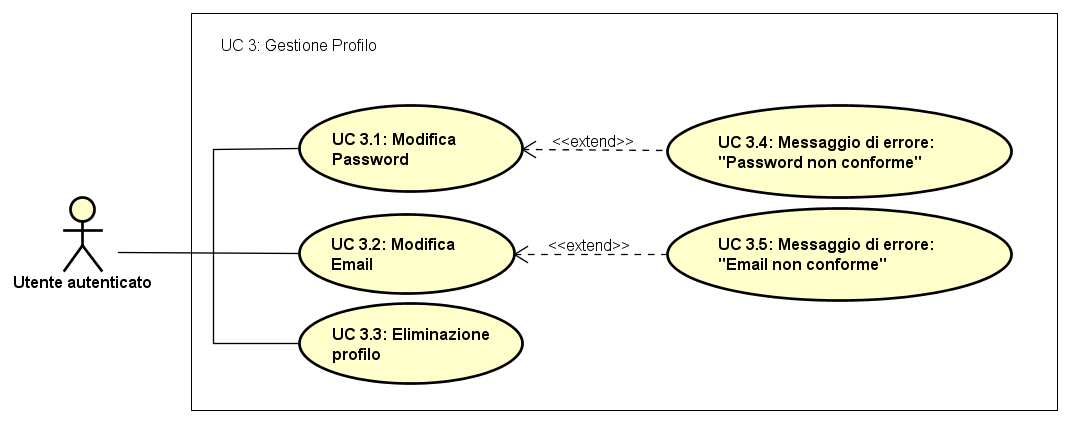
\includegraphics[scale=0.5]{../../Casi D'uso/UC3.png}
\caption{Caso d'uso UC3}
 \end{figure}
\begin{itemize}
\item \textbf{Attori}: \glossaryItem{Utente} autenticato;
\item \textbf{Descrizione}: L'attore può gestire il suo \glossaryItem{Username}, la sua password o il suo indirizzo email;
\item \textbf{Precondizione}: L'attore ha già effettuato l'accesso e l'\glossaryItem{Applicazione} rende disponibile la voce Gestione Profilo nel menù;
\item \textbf{Postcondizione}: L'\glossaryItem{Applicazione} visualizza i dati dell'attore con gli opportuni pulsanti di modifica;
\item \textbf{Scenario principale}:
	\begin{enumerate}\item Modifica Password (UC3.1);\item Modifica Email (UC3.2);\item Eliminazione Profilo (UC3.3);\end{enumerate}
\item \textbf{Scenario alternativo}:
	\begin{enumerate} \item Messaggio di errore: "Password non conforme" (UC3.4);\item Messaggio di errore: "Email non conforme" (UC3.5).
	\end{enumerate}
\end{itemize}
\subsection{UC3.1 - Modifica Password}
\label{ssec:UC3.1}
\begin{itemize}
\item \textbf{Attori}: \glossaryItem{Utente} autenticato;
\item \textbf{Descrizione}: L'attore ha la possibilità di modificare la sua password;
\item \textbf{Precondizione}: L'attore vuole modificare la password;
\item \textbf{Postcondizione}: L'\glossaryItem{Applicazione} modifica la password o restituisce il messaggio d'errore;
\item \textbf{Scenario principale}: L'attore modifica la password;
\item \textbf{Scenari alternativi}: L'attore annulla la modifica della password.
\end{itemize}
\subsection{UC3.2 - Modifica Email}
\label{ssec:UC3.2}
\begin{itemize}
\item \textbf{Attori}: \glossaryItem{Utente} autenticato;
\item \textbf{Descrizione}: L'attore ha la possibilità di modificare la propria email;
\item \textbf{Precondizione}: L'attore vuole modificare l'email;
\item \textbf{Postcondizione}: L'\glossaryItem{Applicazione} aggiorna l'email;
\item \textbf{Scenario principale}: L'attore modifica l'email;
\item \textbf{Scenari alternativi}: L'attore annulla la modifica dell'email.
\end{itemize}
\subsection{UC3.3 - Eliminazione Profilo}
\label{ssec:UC3.3}
\begin{itemize}
\item \textbf{Attori}: \glossaryItem{Utente} autenticato;
\item \textbf{Descrizione}: L'attore può eliminare il profilo, cancellando ogni tipo di personalizzazione da lui creata;
\item \textbf{Precondizione}: L'\glossaryItem{Applicazione} permette l'eliminazione del profilo;
\item \textbf{Postcondizione}: L'\glossaryItem{Applicazione} ha cancellato a cascata ogni informazione legata a tale profilo ed essa non è più recuperabile;
\item \textbf{Scenario principale}: L'attore elimina il proprio profilo e tutti i dati contenuti in esso;
\item \textbf{Scenari alternativi}: L'attore annulla la cancellazione del profilo.
\end{itemize}
\subsection{UC3.4 - Messaggio di errore: "Password non conforme"}
\label{ssec:UC3.4}
\begin{itemize}
\item \textbf{Attori}: \glossaryItem{Utente} autenticato;
\item \textbf{Descrizione}: L'attore può inserire una password non conforme e gli viene quindi comunicato l'errore;
\item \textbf{Precondizione}: L'\glossaryItem{Applicazione} è pronta e l'\glossaryItem{Utente} modifica la password;
\item \textbf{Postcondizione}: L'attore ha inserito una password non conforme e ha ricevuto la comunicazione dell'errore;
\item \textbf{Scenario principale}: L'attore viene avvisato che la password non è conforme.
\end{itemize}
\subsection{UC3.5 - Messaggio di errore: "Email non conforme"}
\label{ssec:UC3.5}
\begin{itemize}
\item \textbf{Attori}: \glossaryItem{Utente} autenticato;
\item \textbf{Descrizione}: L'attore può inserire l'email con una sintassi non valida e gli viene quindi comunicato l'errore;
\item \textbf{Precondizione}: L'appplicazione è pronta e l'attore intende modificare l'email;
\item \textbf{Postcondizione}: L'attore ha inserito un'email non conforme e ha ricevuto la comunicazione dell'errore;
\item \textbf{Scenario principale}: L'attore viene avvisato che l'email non è conforme.
\end{itemize}
\newpage
\subsection{UC4 - Logout}
\label{ssec:UC4}
\begin{itemize}
\item \textbf{Attori}: \glossaryItem{Utente} autenticato;
\item \textbf{Descrizione}: L'attore può effettuare il logout dal suo profilo;
\item \textbf{Precondizione}: L’\glossaryItem{Applicazione} mette a disposizione dell’attore la possibilità di logout;
\item \textbf{Postcondizione}: L'\glossaryItem{Applicazione} effettua il logout dell'attore;
\item \textbf{Scenario principale}: L'attore effettua il logout.
\end{itemize}
\newpage
\subsection{UC5 - Gestione Progetti}
\label{ssec:UC5}
\begin{figure}[h!]
\centering
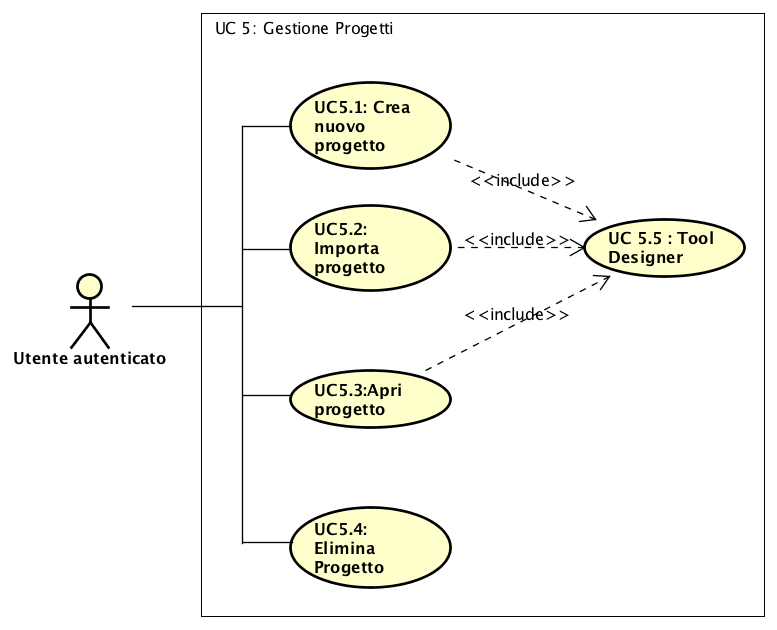
\includegraphics[scale=0.5]{../../Casi D'uso/UC5.png}
\caption{Caso d'uso UC5}
 \end{figure}
\begin{itemize}
\item \textbf{Attori}: \glossaryItem{Utente} autenticato;
\item \textbf{Descrizione}: L’ attore ha la possibilità di aggiungere un nuovo progetto e di aprire o modificare un progetto già esistente;
\item \textbf{Precondizione}: L'\glossaryItem{Applicazione} è pronta e l'attore intende gestire un progetto;
\item \textbf{Postcondizione}: L’ \glossaryItem{Applicazione} visualizza la lista delle funzionalità disponibili;
\item \textbf{Scenario principale}: \begin{enumerate}\item Aggiunta Progetto (UC5.1);\item Apertura progetto (UC5.2);\item Eliminazione Progetto (UC5.3).
 \end{enumerate}
\end{itemize}
\newpage
\subsection{UC5.1 - Aggiunta Progetto}
\label{ssec:UC5.1}
\begin{figure}[h!]
\centering
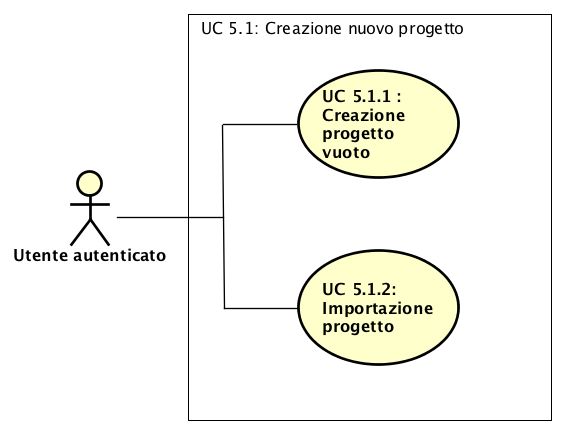
\includegraphics[scale=0.5]{../../Casi D'uso/UC5.1.png}
\caption{Caso d'uso UC5.1}
 \end{figure}
\begin{itemize}
\item \textbf{Attori}: \glossaryItem{Utente} autenticato;
\item \textbf{Descrizione}: L’attore ha la possibilità di creare o importare un progetto;
\item \textbf{Precondizione}: L’attore vuole aggiungere un nuovo progetto alla lista;
\item \textbf{Postcondizione}: L’\glossaryItem{Applicazione} apre la lista dei modi per aggiungere un progetto;
\item \textbf{Scenario principale}: \begin{enumerate}\item Creazione Progetto vuoto (UC5.1.1);\item Importazione Progetto (UC5.1.2);
 \end{enumerate}
\item \textbf{Scenari alternativi}: L'attore decide di non aggiungere un nuovo progetto.
\end{itemize}
\subsection{UC5.1.1 - Creazione Progetto vuoto}
\label{ssec:UC5.1.1}
\begin{itemize}
\item \textbf{Attori}: \glossaryItem{Utente} autenticato;
\item \textbf{Descrizione}: L'attore può creare un nuovo progetto;
\item \textbf{Precondizione}: L'attore vuole creare un progetto vuoto;
\item \textbf{Postcondizione}: L'\glossaryItem{Applicazione} crea un nuovo progetto vuoto;
\item \textbf{Scenario principale}: L'attore crea un nuovo progetto;
\item \textbf{Scenari alternativi}: L'attore annulla la creazione del nuovo progetto.
\end{itemize}
\newpage
\subsection{UC5.1.2 - Importazione Progetto}
\label{ssec:UC5.1.2}
\begin{itemize}
\item \textbf{Attori}: \glossaryItem{Utente} autenticato;
\item \textbf{Descrizione}: L'attore può importare un progetto precedentemente esportato dall'applicazione, presente nel proprio dispositivo;
\item \textbf{Precondizione}: L'attore vuole importare un progetto, ha a disposizione un progetto valido;
\item \textbf{Postcondizione}: L'\glossaryItem{Applicazione} importa il progetto richiesto;
\item \textbf{Scenario principale}: L'attore importa un progetto;
\item \textbf{Scenari alternativi}: L'attore decide di non importare nessun progetto.
\end{itemize}
\subsection{UC5.2 - Apertura progetto}
\label{ssec:UC5.2}
\begin{itemize}
\item \textbf{Attori}: \glossaryItem{Utente} autenticato.
\item \textbf{Descrizione}: L’attore ha la possibilità di aprire un progetto precedentemente salvato.;
\item \textbf{Precondizione}: L’\glossaryItem{Applicazione} rende disponibile la lista dei progetti dell'attore;
\item \textbf{Postcondizione}: L’\glossaryItem{Applicazione} apre il progetto selezionato;
\item \textbf{Scenario principale}: L'attore apre un progetto salvato precedentemente.
\end{itemize}
\subsection{UC5.3 - Eliminazione Progetto}
\label{ssec:UC5.3}
\begin{itemize}
\item \textbf{Attori}: \glossaryItem{Utente} autenticato;
\item \textbf{Descrizione}: L'attore ha la possibilità di eliminare un progetto precedentemente salvato;
\item \textbf{Precondizione}: L’\glossaryItem{Applicazione} rende disponibile la lista dei progetti salvati dall'attore;
\item \textbf{Postcondizione}: L’\glossaryItem{Applicazione} elimina il progetto selezionato;
\item \textbf{Scenario principale}: L'attore elimina un progetto precedentemente salvato.
\end{itemize}
\newpage
\subsection{UC6 - Tool Designer}
\label{ssec:UC6}
\begin{figure}[h!]
\centering
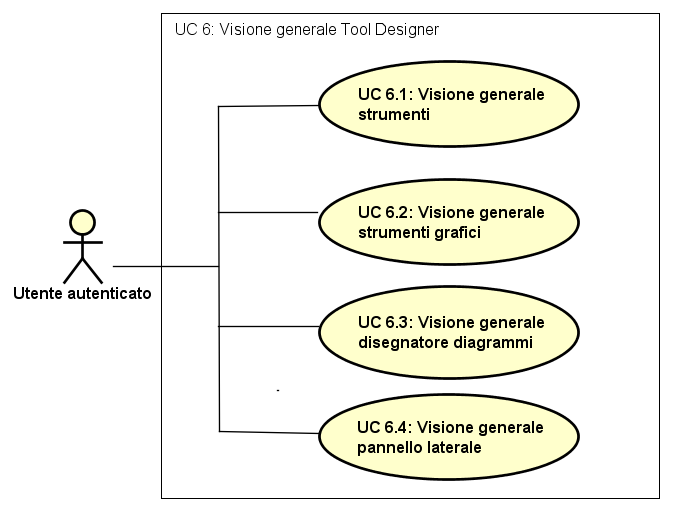
\includegraphics[scale=0.5]{../../Casi D'uso/UC6.png}
\caption{Caso d'uso UC6}
 \end{figure}
\begin{itemize}
\item \textbf{Attori}: \glossaryItem{Utente} autenticato;
\item \textbf{Descrizione}: L'\glossaryItem{Applicazione} visualizza l'editor dei \glossaryItem{Diagrammi};
\item \textbf{Precondizione}: L' attore ha effettuato l'accesso;
\item \textbf{Postcondizione}: L'\glossaryItem{Applicazione} visualizza la finestra;
\item \textbf{Scenario principale}: \begin{enumerate}\item Menù (UC6.1);\item Barra degli strumenti (UC6.2);\item Disegnatore \glossaryItem{Diagrammi} (UC6.3);\item Pannello laterale (UC6.4).
 \end{enumerate}
\end{itemize}
\newpage
\subsection{UC6.1 - Menù}
\label{ssec:UC6.1}
\begin{figure}[h!]
\centering
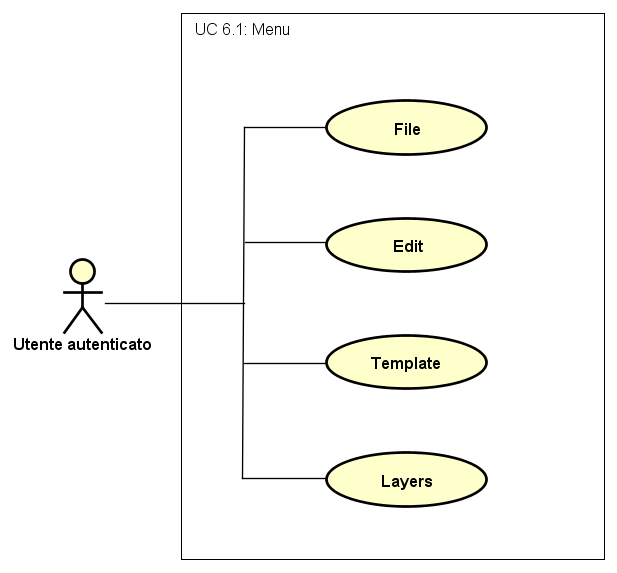
\includegraphics[scale=0.5]{../../Casi D'uso/UC6.1.png}
\caption{Caso d'uso UC6.1}
 \end{figure}
\begin{itemize}
\item \textbf{Attori}: \glossaryItem{Utente} autenticato;
\item \textbf{Descrizione}: L’attore può accedere alle voci File, edit, tool,
layers appartenenti al menù del Tool \glossaryItem{Designer};
\item \textbf{Precondizione}: L’\glossaryItem{Applicazione} offre all’\glossaryItem{Utente} una barra dei menù;
\item \textbf{Postcondizione}: L’\glossaryItem{Applicazione}, a seconda dell’operazione richiesta dall’\glossaryItem{Utente},
svolge le sue funzioni;
\item \textbf{Scenario principale}: \begin{enumerate}\item File (UC6.1.1);\item Edit (UC6.1.2);\item \glossaryItem{Template} (UC6.1.3);\item layers (UC6.1.4).
 \end{enumerate}
\end{itemize}
\newpage
\subsection{UC6.1.1 - File}
\label{ssec:UC6.1.1}
\begin{figure}[h!]
\centering
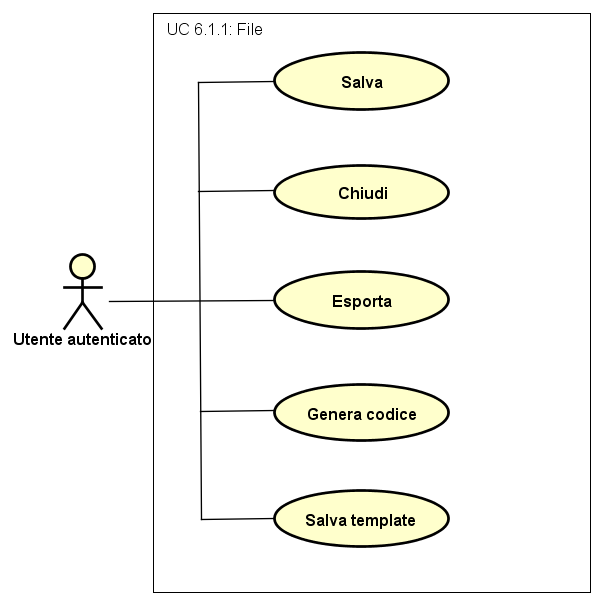
\includegraphics[scale=0.5]{../../Casi D'uso/UC6.1.1.png}
\caption{Caso d'uso UC6.1.1}
 \end{figure}
\begin{itemize}
\item \textbf{Attori}: \glossaryItem{Utente} autenticato;
\item \textbf{Descrizione}: L’attore può accedere alle voci salva, chiudi, esporta, genera \glossaryItem{Codice} e salva \glossaryItem{Template} appartenenti alla voce File del menù;
\item \textbf{Precondizione}: L’\glossaryItem{Applicazione} offre all’attore la voce File nella barra dei menù;
\item \textbf{Postcondizione}: L’\glossaryItem{Applicazione}, a seconda dell’operazione richiesta dall’\glossaryItem{Utente},
svolge le sue funzioni;
\item \textbf{Scenario principale}: \begin{enumerate}\item Salvataggio (UC6.1.1.1);\item Chiusura (UC6.1.1.2);\item Esportazione (UC6.1.1.3);\item Genera \glossaryItem{Codice} (UC6.1.1.4);\item Salvataggio \glossaryItem{Template} (UC6.1.1.5).
 \end{enumerate}
\end{itemize}
\newpage
\subsection{UC6.1.1.1 - Salvataggio}
\label{ssec:UC6.1.1.1}
\begin{itemize}
\item \textbf{Attori}: \glossaryItem{Utente} autenticato;
\item \textbf{Descrizione}: L’attore può salvare il suo progetto nello stato corrente;
\item \textbf{Precondizione}: L’attore ha aperto un progetto;
\item \textbf{Postcondizione}: L’\glossaryItem{Applicazione} salva il progetto nello stato corrente;
\item \textbf{Scenario principale}: L'attore salva il progetto nello stato corrente.
\end{itemize}
\subsection{UC6.1.1.2 - Chiusura}
\label{ssec:UC6.1.1.2}
\begin{itemize}
\item \textbf{Attori}: \glossaryItem{Utente} autenticato;
\item \textbf{Descrizione}: L’attore può chiudere il progetto corrente;
\item \textbf{Precondizione}: L'attore ha aperto un progetto;
\item \textbf{Postcondizione}: L’\glossaryItem{Applicazione} chiude il progetto corrente;
\item \textbf{Scenario principale}: L'attore chiude il progetto corrente.
\end{itemize}
\subsection{UC6.1.1.3 - Esportazione}
\label{ssec:UC6.1.1.3}
\begin{itemize}
\item \textbf{Attori}: \glossaryItem{Utente} autenticato;
\item \textbf{Descrizione}: L’attore può esportare il progetto corrente per possederne una copia digitale;
\item \textbf{Precondizione}: L’attore ha un progetto aperto;
\item \textbf{Postcondizione}: L’\glossaryItem{Applicazione} esporta il progetto in un formato compresso;
\item \textbf{Scenario principale}: L'attore esporta il progetto corrente.
\end{itemize}
\subsection{UC6.1.1.4 - Genera codice}
\label{ssec:UC6.1.1.4}
\begin{itemize}
\item \textbf{Attori}: \glossaryItem{Utente} autenticato;
\item \textbf{Descrizione}: L’attore può generare il \glossaryItem{Codice} relativo all’\glossaryItem{UML} prodotto;
\item \textbf{Precondizione}: L’attore vuole generare il \glossaryItem{Codice} dai suoi \glossaryItem{Diagrammi} \glossaryItem{UML} in linguaggio Java;
\item \textbf{Postcondizione}: L’\glossaryItem{Applicazione} genera il \glossaryItem{Codice} relativo al disegno \glossaryItem{UML};
\item \textbf{Scenario principale}: L'attore richiede la generazione del codice.
\end{itemize}
\subsection{UC6.1.1.5 - Salvataggio template}
\label{ssec:UC6.1.1.5}
\begin{itemize}
\item \textbf{Attori}: \glossaryItem{Utente} autenticato;
\item \textbf{Descrizione}: L’attore ha la possibilità di salvare determinate \glossaryItem{Classi} o gerarchie, aggiungendole così alla lista di \glossaryItem{Template} già salvati;
\item \textbf{Precondizione}: L’\glossaryItem{Applicazione} offre all’attore la voce salva \glossaryItem{Template}, sottovoce di File nel menù, solamente se sono state create una o più \glossaryItem{Classi}, ed ognuna di esse ha un commento che le identifica;
\item \textbf{Postcondizione}: Viene aggiunto alla lista dei \glossaryItem{Template} il \glossaryItem{Template} desiderato;
\item \textbf{Scenario principale}: L'attore salva determinate classi o gerarchie tra i propri Template.
\end{itemize}
\newpage
\subsection{UC6.1.2 - Edit}
\label{ssec:UC6.1.2}
\begin{figure}[h!]
\centering
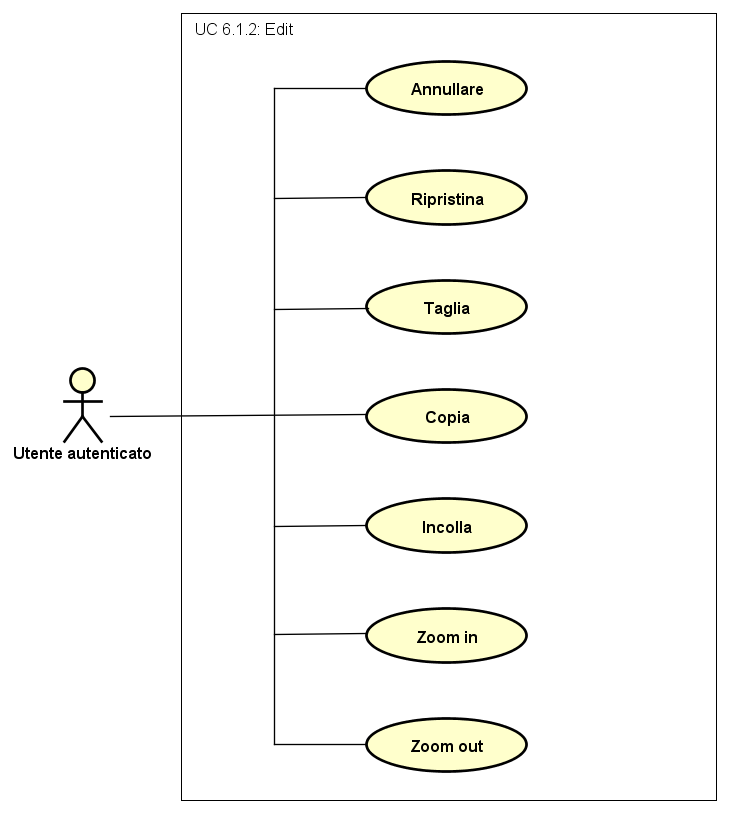
\includegraphics[scale=0.5]{../../Casi D'uso/UC6.1.2.png}
\caption{Caso d'uso UC6.1.2}
 \end{figure}
\begin{itemize}
\item \textbf{Attori}: \glossaryItem{Utente} autenticato;
\item \textbf{Descrizione}: L’attore può accedere alle voci annulla, ripristina, taglia, copia, incolla, \glossaryItem{Zoom} in e \glossaryItem{Zoom} out appartenenti alla voce edit del menù;
\item \textbf{Precondizione}: L'attore ha aperto un progetto;
\item \textbf{Postcondizione}: L’\glossaryItem{Applicazione} visualizza la lista delle funzionalità disponibili;
\item \textbf{Scenario principale}: \begin{enumerate}\item Annulla (UC6.1.2.1);\item Ripristina (UC6.1.2.2);\item Taglia (UC6.1.2.3);\item Copia (UC6.1.2.4);\item Incolla (UC6.1.2.5);\item \glossaryItem{Zoom} in (UC6.1.2.6);\item \glossaryItem{Zoom} out (UC6.1.2.7).
 \end{enumerate}
\end{itemize}
\subsection{UC6.1.2.1 - Annulla}
\label{ssec:UC6.1.2.1}
\begin{itemize}
\item \textbf{Attori}: \glossaryItem{Utente} autenticato;
\item \textbf{Descrizione}: L’attore può tornare allo stato precedente l’ultima modifica;
\item \textbf{Precondizione}: L'attore ha un progetto aperto e ne ha effettuato una modifica;
\item \textbf{Postcondizione}: L’\glossaryItem{Applicazione} torna allo stato precedente l’ultima modifica;
\item \textbf{Scenario principale}: L'attore annulla l'ultima modifica applicata.
\end{itemize}
\subsection{UC6.1.2.2 - Ripristina}
\label{ssec:UC6.1.2.2}
\begin{itemize}
\item \textbf{Attori}: \glossaryItem{Utente} autenticato;
\item \textbf{Descrizione}: L’attore può ripristinare le modifiche effettuate successivamente allo stato attuale;
\item \textbf{Precondizione}: L’attore ha un progetto aperto ed ha annullato una modifica (UC 6.1.2.1);
\item \textbf{Postcondizione}: L’\glossaryItem{Applicazione} torna allo stato precedente l’ultima modifica;
\item \textbf{Scenario principale}: L'attore ripristina le modifiche effettuate successivamente allo stato attuale.
\end{itemize}
\subsection{UC6.1.2.3 - Taglia}
\label{ssec:UC6.1.2.3}
\begin{itemize}
\item \textbf{Attori}: \glossaryItem{Utente} autenticato;
\item \textbf{Descrizione}: L’attore può "tagliare" un determinato elemento del progetto;
\item \textbf{Precondizione}: L’attore ha un progetto aperto ed ha selezionato almeno un elemento dei \glossaryItem{Diagrammi};
\item \textbf{Postcondizione}: L’\glossaryItem{Applicazione} taglia l’elemento selezionato;
\item \textbf{Scenario principale}: L'attore 'taglia' un determinato elemento del progetto.
\end{itemize}
\subsection{UC6.1.2.4 - Copia}
\label{ssec:UC6.1.2.4}
\begin{itemize}
\item \textbf{Attori}: \glossaryItem{Utente} autenticato;
\item \textbf{Descrizione}: L’attore può "copiare" un determinato elemento del progetto.;
\item \textbf{Precondizione}: L’attore ha un progetto aperto ed ha selezionato almeno un elemento dei \glossaryItem{Diagrammi};
\item \textbf{Postcondizione}: L’\glossaryItem{Applicazione} copia l’elemento selezionato;
\item \textbf{Scenario principale}: L'attore 'copia' un determinato elemento del progetto.
\end{itemize}
\subsection{UC6.1.2.5 - Incolla}
\label{ssec:UC6.1.2.5}
\begin{itemize}
\item \textbf{Attori}: \glossaryItem{Utente} autenticato;
\item \textbf{Descrizione}: L’attore può "incollare" un elemento precedentemente tagliato o copiato;
\item \textbf{Precondizione}: L’attore ha un progetto aperto ed ha selezionato almeno un elemento dei \glossaryItem{Diagrammi};
\item \textbf{Postcondizione}: L’\glossaryItem{Applicazione} inserisce l’elemento designato;
\item \textbf{Scenario principale}: L'attore 'incolla' un determinato elemento del progetto.
\end{itemize}
\subsection{UC6.1.2.6 - \glossaryItem{Zoom} in}
\label{ssec:UC6.1.2.6}
\begin{itemize}
\item \textbf{Attori}: \glossaryItem{Utente} autenticato;
\item \textbf{Descrizione}: L’attore può ingrandire la visualizzazione di una determinata sezione;
\item \textbf{Precondizione}: L’attore ha un progetto aperto;
\item \textbf{Postcondizione}: L’\glossaryItem{Applicazione} ingrandisce gli elementi nella finestra del disegnatore dei \glossaryItem{Diagrammi} (UC 6.3);
\item \textbf{Scenario principale}: L'attore ingrandisce la visualizzazione di una determinata sezione.
\end{itemize}
\subsection{UC6.1.2.7 - \glossaryItem{Zoom} out}
\label{ssec:UC6.1.2.7}
\begin{itemize}
\item \textbf{Attori}: \glossaryItem{Utente} autenticato;
\item \textbf{Descrizione}: L’attore può rimpicciolire la visualizzazione di una determinata sezione;
\item \textbf{Precondizione}: L’attore ha un progetto aperto;
\item \textbf{Postcondizione}: L’\glossaryItem{Applicazione} rimpicciolisce gli elementi nella finestra del disegnatore dei \glossaryItem{Diagrammi} (UC 6.3);
\item \textbf{Scenario principale}: L'attore rimpicciolisce la visualizzazione di una determinata sezione.
\end{itemize}
\newpage
\subsection{UC6.1.3 - Template}
\label{ssec:UC6.1.3}
\begin{figure}[h!]
\centering
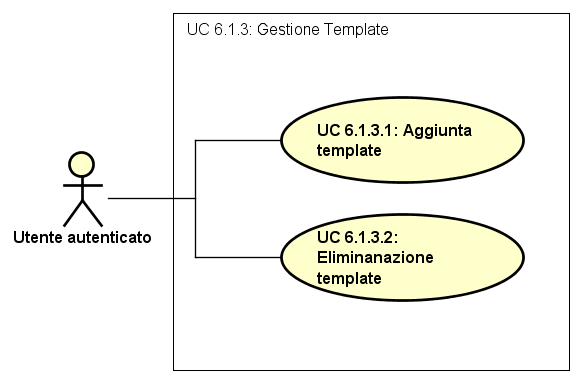
\includegraphics[scale=0.5]{../../Casi D'uso/UC6.1.3.png}
\caption{Caso d'uso UC6.1.3}
 \end{figure}
\begin{itemize}
\item \textbf{Attori}: \glossaryItem{Utente} autenticato;
\item \textbf{Descrizione}: L’attore può accedere alla visualizzazione della lista dei \glossaryItem{Template}. I \glossaryItem{Template} visualizzati comprendono sia quelli già dati dagli sviluppatore, sia i propri \glossaryItem{Template};
\item \textbf{Precondizione}: L’attore ha aperto un progetto;
\item \textbf{Postcondizione}: L'\glossaryItem{Applicazione} ha aperto una finestra dove viene visualizzata la lista dei \glossaryItem{Template};
\item \textbf{Scenario principale}: \begin{enumerate}\item Aggiunta \glossaryItem{Template} (UC6.1.3.1);\item Eliminazione \glossaryItem{Template} (UC6.1.3.2).
 \end{enumerate}
\end{itemize}
\subsection{UC6.1.3.1 - Aggiunta template}
\label{ssec:UC6.1.3.1}
\begin{itemize}
\item \textbf{Attori}: \glossaryItem{Utente} autenticato;
\item \textbf{Descrizione}: L'attore può inserire nella finestra del disegnatore dei \glossaryItem{Diagrammi} (UC 6.3) il \glossaryItem{Template} selezionato;
\item \textbf{Precondizione}: L'attore ha aperto la finestra di gestione dei \glossaryItem{Template};
\item \textbf{Postcondizione}: L'attore aggiunge il \glossaryItem{Template} selezionato nella finestra del disegnatore dei \glossaryItem{Diagrammi}(UC 6.3);
\item \textbf{Scenario principale}: L'attore inserisce nel disegnatore dei diagrammi il template selezionato;
\item \textbf{Scenari alternativi}: L'attore chiude la finestra di gestione \glossaryItem{Template} (UC 6.1.3) e non viene effettuata nessuna operazione.
\end{itemize}
\subsection{UC6.1.3.2 - Eliminazione template}
\label{ssec:UC6.1.3.2}
\begin{itemize}
\item \textbf{Attori}: \glossaryItem{Utente} autenticato;
\item \textbf{Descrizione}: L'attore può eliminare dalla lista il \glossaryItem{Template} selezionato;
\item \textbf{Precondizione}: L'attore ha aperto la finestra di gestione dei \glossaryItem{Template} (UC 6.1.3);
\item \textbf{Postcondizione}: Il \glossaryItem{Template} selezionato viene rimosso dalla lista;
\item \textbf{Scenario principale}: L'attore elimina dalla lista il template selezionato;
\item \textbf{Scenari alternativi}: L'attore chiude la finestra di gestione \glossaryItem{Template} (UC 6.1.3) e non viene effettuata nessuna operazione.
\end{itemize}
\newpage
\subsection{UC6.1.4 - layers}
\label{ssec:UC6.1.4}
\begin{figure}[h!]
\centering
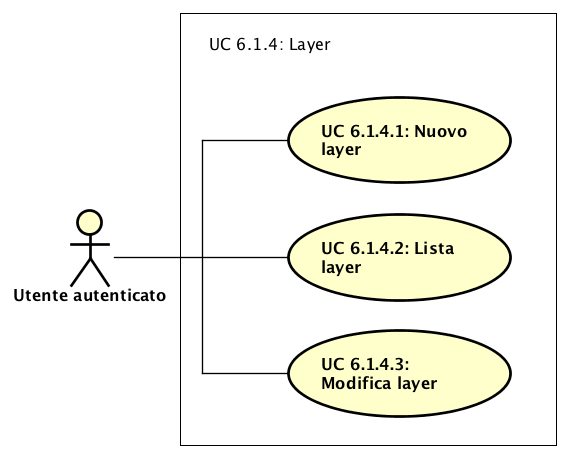
\includegraphics[scale=0.5]{../../Casi D'uso/UC6.1.4.png}
\caption{Caso d'uso UC6.1.4}
 \end{figure}
\begin{itemize}
\item \textbf{Attori}: \glossaryItem{Utente} autenticato;
\item \textbf{Descrizione}: L’attore  può accedere alla visualizzazione della lista dei layers. Può inoltre creare nuovi layer oppure rinominarne o eliminarne di già esistenti;
\item \textbf{Precondizione}: L’attore ha un progetto aperto;
\item \textbf{Postcondizione}: L'\glossaryItem{Applicazione} visualizza la lista delle funzionalità disponibili sui layer;
\item \textbf{Scenario principale}: \begin{enumerate}\item Nuovo layer (UC6.1.4.1);\item Lista layer (UC6.1.4.2);\item Modifica layer (UC6.1.4.3).
 \end{enumerate}
\end{itemize}
\subsection{UC6.1.4.1 - Nuovo layer}
\label{ssec:UC6.1.4.1}
\begin{itemize}
\item \textbf{Attori}: \glossaryItem{Utente} autenticato;
\item \textbf{Descrizione}: L'attore crea un nuovo layer a cui è possibile assegnare delle \glossaryItem{Classi};
\item \textbf{Precondizione}: L'attore ha aperto la finestra di gestione dei layer;
\item \textbf{Postcondizione}: L'attore ha aggiunto un nuovo layer assegnandogli il nome desiderato;
\item \textbf{Scenario principale}: L'attore crea un nuovo layer.
\end{itemize}
\subsection{UC6.1.4.2 - Lista layer}
\label{ssec:UC6.1.4.2}
\begin{itemize}
\item \textbf{Attori}: \glossaryItem{Utente} autenticato;
\item \textbf{Descrizione}: L'attore seleziona il layer di cui desidera visualizzare le \glossaryItem{Classi} che gli sono state assegnate;
\item \textbf{Precondizione}: L'attore ha aperto la finestra di gestione dei layer;
\item \textbf{Postcondizione}: L'attore ha visualizzato le \glossaryItem{Classi} assegnate al layer desiderato;
\item \textbf{Scenario principale}: L'attore seleziona il layer desiderato dalla lista.
\end{itemize}
\newpage
\subsection{UC6.1.4.3 - Modifica layer}
\label{ssec:UC6.1.4.3}
\begin{figure}[h!]
\centering
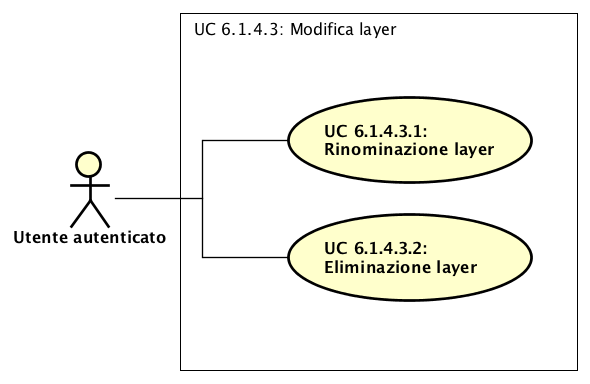
\includegraphics[scale=0.5]{../../Casi D'uso/UC6.1.4.3.png}
\caption{Caso d'uso UC6.1.4.3}
 \end{figure}
\begin{itemize}
\item \textbf{Attori}: \glossaryItem{Utente} autenticato;
\item \textbf{Descrizione}: L'attore desidera rinominare oppure eliminare un layer tra quelli esistenti;
\item \textbf{Precondizione}: L'attore ha aperto la finestra di gestione dei layer;
\item \textbf{Postcondizione}: L'\glossaryItem{Applicazione} apre la finestra di gestione dei layer;
\item \textbf{Scenario principale}: \begin{enumerate}\item Rinominazione layer (UC6.1.4.3.1);\item Eliminazione layer (UC6.1.4.3.2).
 \end{enumerate}
\end{itemize}
\subsection{UC6.1.4.3.1 - Rinominazione layer}
\label{ssec:UC6.1.4.3.1}
\begin{itemize}
\item \textbf{Attori}: \glossaryItem{Utente} autenticato;
\item \textbf{Descrizione}: L'attore desidera rinominare un layer tra quelli esistenti;
\item \textbf{Precondizione}: L'attore seleziona il layer da rinominare;
\item \textbf{Postcondizione}: L'attore ha modificato il nome del layer che intendeva modificare, mantenendo tutte le \glossaryItem{Classi} associate;
\item \textbf{Scenario principale}: L'attore rinomina un layer esistente.
\end{itemize}
\subsection{UC6.1.4.3.2 - Eliminazione layer}
\label{ssec:UC6.1.4.3.2}
\begin{itemize}
\item \textbf{Attori}: \glossaryItem{Utente} autenticato;
\item \textbf{Descrizione}: L'attore desidera eliminare un layer tra quelli esistenti;
\item \textbf{Precondizione}: L'attore seleziona un layer;
\item \textbf{Postcondizione}: L'\glossaryItem{Applicazione} ha eliminato il layer che intendeva modificare e tutte le \glossaryItem{Classi} assegnate a tale layer, se ce n'erano, non risultano più assegnate a nessun layer;
\item \textbf{Scenario principale}: L'attore elimina un layer esistente.
\end{itemize}
\newpage
\subsection{UC6.2 - Barra degli strumenti}
\label{ssec:UC6.2}
\begin{figure}[h!]
\centering
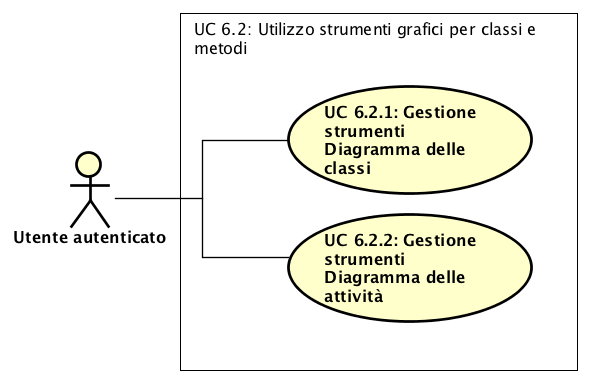
\includegraphics[scale=0.5]{../../Casi D'uso/UC6.2.png}
\caption{Caso d'uso UC6.2}
 \end{figure}
\begin{itemize}
\item \textbf{Attori}: \glossaryItem{Utente} autenticato;
\item \textbf{Descrizione}: L'\glossaryItem{Applicazione} visualizza la barra degli strumenti grafici;
\item \textbf{Precondizione}: L'attore ha effettuato l'accesso;
\item \textbf{Postcondizione}: L'\glossaryItem{Applicazione} visualizza la barra degli strumenti grafici;
\item \textbf{Scenario principale}: \begin{enumerate}\item Strumenti delle \glossaryItem{Classi} (UC6.2.1);\item Strumenti \glossaryItem{Diagramma delle Attività} (UC6.2.2).
 \end{enumerate}
\end{itemize}
\newpage
\subsection{UC6.2.1 - Strumenti delle classi}
\label{ssec:UC6.2.1}
\begin{figure}[h!]
\centering
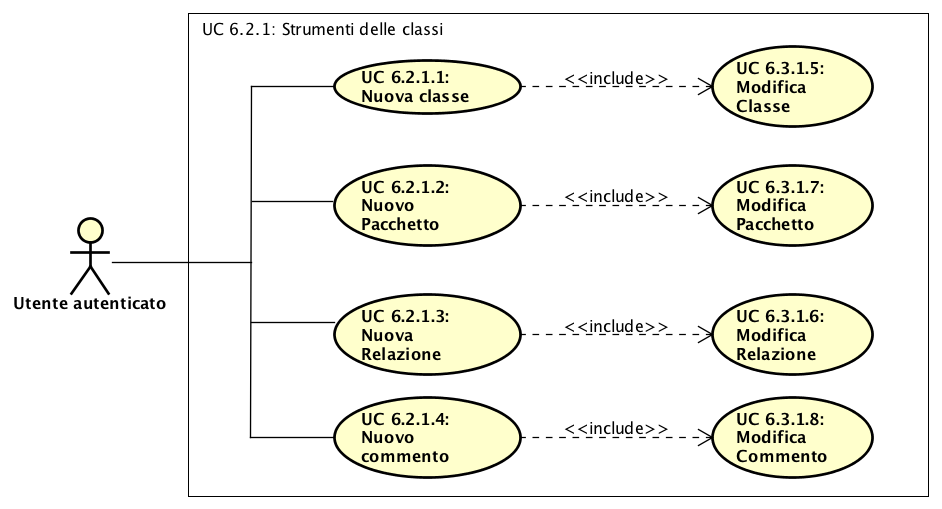
\includegraphics[scale=0.5]{../../Casi D'uso/UC6.2.1.png}
\caption{Caso d'uso UC6.2.1}
 \end{figure}
\begin{itemize}
\item \textbf{Attori}: \glossaryItem{Utente} autenticato;
\item \textbf{Descrizione}: L'attore, per la creazione di un \glossaryItem{Diagramma delle Classi} ha la possibilità di selezionare una nuova \glossaryItem{Classe}, inserire un \glossaryItem{Package} per raggruppare delle \glossaryItem{Classi} o inserire delle relazioni tra le \glossaryItem{Classi};
\item \textbf{Precondizione}: L'attore ha aperto un progetto;
\item \textbf{Postcondizione}: L'\glossaryItem{Applicazione} visualizza gli strumenti per disegnare le \glossaryItem{Classi};
\item \textbf{Scenario principale}: \begin{enumerate}\item Nuova \glossaryItem{Classe} (UC6.2.1.1);\item Nuovo Pacchetto (UC6.2.1.2);\item Nuova Relazione (UC6.2.1.3);\item Nuovo commento (UC6.2.1.4);
 \end{enumerate}
 \item \textbf{Inclusioni}: \begin{itemize}
 	\item \textbf{ Modifica \glossaryItem{Classe} (UC 6.3.1.5)};
 	\item \textbf{ Modifica Pacchetto (UC 6.3.1.7)};
 	\item \textbf{ Modifica Relazione (UC 6.3.1.6)};
 	\item \textbf{ Modifica Commento (UC 6.3.1.8)}.
 \end{itemize}
\end{itemize}
\subsection{UC6.2.1.1 - Nuova Classe}
\label{ssec:UC6.2.1.1}
\begin{itemize}
\item \textbf{Attori}: \glossaryItem{Utente} autenticato:
\item \textbf{Descrizione}: L'attore ha la possibilità di inserire il disegno rappresentante una \glossaryItem{Classe} nello standard \glossaryItem{UML} con i relativi campi compilati;
\item \textbf{Precondizione}: L'attore ha un progetto aperto;
\item \textbf{Postcondizione}: Viene rappresentato il disegno della \glossaryItem{Classe} e vengono salvati i dati contenuti in essa;
\item \textbf{Scenario principale}: L'attore inserisce il disegno di una nuova classe.
\end{itemize}
\subsection{UC6.2.1.2 - Nuovo Pacchetto}
\label{ssec:UC6.2.1.2}
\begin{itemize}
\item \textbf{Attori}: \glossaryItem{Utente} autenticato;
\item \textbf{Descrizione}: L'attore ha la possibilità di inserire il disegno rappresentante un \glossaryItem{Package} nello standard \glossaryItem{UML};
\item \textbf{Precondizione}: L'attore ha un progetto aperto;
\item \textbf{Postcondizione}: L'\glossaryItem{Applicazione} rappresentata il disegno del \glossaryItem{Package} e vengono salvati i relativi dati;
\item \textbf{Scenario principale}: L'attore inserisce il disegno di una nuova package.
\end{itemize}
\newpage
\subsection{UC6.2.1.3 - Nuova Relazione}
\label{ssec:UC6.2.1.3}
\begin{figure}[h!]
\centering
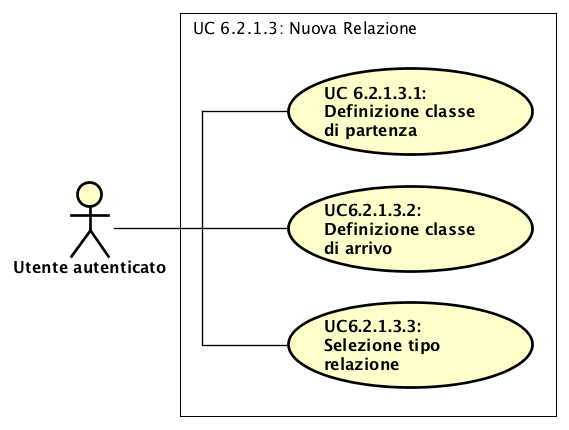
\includegraphics[scale=0.5]{../../Casi D'uso/UC6.2.1.3.png}
\caption{Caso d'uso UC6.2.1.3}
 \end{figure}
\begin{itemize}
\item \textbf{Attori}: \glossaryItem{Utente} autenticato;
\item \textbf{Descrizione}: L'\glossaryItem{Applicazione} fornisce una lista di relazioni tra le \glossaryItem{Classi};
\item \textbf{Precondizione}: L'attore ha aperto un progetto;
\item \textbf{Postcondizione}: L'\glossaryItem{Applicazione} fornisce una lista di relazioni tra le \glossaryItem{Classi};
\item \textbf{Scenario principale}: \begin{enumerate}\item Definizione \glossaryItem{Classe} di partenza (UC6.2.1.3.1);\item Definizione \glossaryItem{Classe} di arrivo (UC6.2.1.3.2);\item Selezione tipo relazione (UC6.2.1.3.3).
 \end{enumerate}
\end{itemize}
\subsection{UC6.2.1.3.1 - Definizione \glossaryItem{Classe} di partenza}
\label{ssec:UC6.2.1.3.1}
\begin{itemize}
\item \textbf{Attori}: \glossaryItem{Utente} autenticato;
\item \textbf{Descrizione}: Viene definito il punto di partenza dell'associazione;
\item \textbf{Precondizione}: Esiste almeno una \glossaryItem{Classe};
\item \textbf{Postcondizione}: L'\glossaryItem{Applicazione} associa il disegno dell'assegnazione alla relativa \glossaryItem{Classe};
\item \textbf{Scenario principale}: L'attore definisce il punto di partenza dell'associazione.
\end{itemize}
\subsection{UC6.2.1.3.2 - Definizione \glossaryItem{Classe} di arrivo}
\label{ssec:UC6.2.1.3.2}
\begin{itemize}
\item \textbf{Attori}: \glossaryItem{Utente} autenticato;
\item \textbf{Descrizione}: Viene definito il punto di arrivo dell'associazione;
\item \textbf{Precondizione}: Esiste almeno una \glossaryItem{Classe};
\item \textbf{Postcondizione}: L'\glossaryItem{Applicazione} associa il disegno dell'assegnazione alla relativa \glossaryItem{Classe} di destinazione;
\item \textbf{Scenario principale}: L'attore definisce il punto di arrivo dell'associazione.
\end{itemize}
\subsection{UC6.2.1.3.3 - Selezione tipo relazione}
\label{ssec:UC6.2.1.3.3}
\begin{itemize}
\item \textbf{Attori}: \glossaryItem{Utente} autenticato;
\item \textbf{Descrizione}: L'attore seleziona il tipo di relazione tra: dipendenza, associazione, gerarchia;
\item \textbf{Precondizione}: L'\glossaryItem{Applicazione} visualizza il form per l'inserimento dei dati;
\item \textbf{Postcondizione}: L'\glossaryItem{Applicazione} ha registrato i dati inseriti;
\item \textbf{Scenario principale}: L'attore seleziona il tipo di relazione.
\end{itemize}
\subsection{UC6.2.1.4 - Nuovo commento}
\label{ssec:UC6.2.1.4}
\begin{itemize}
\item \textbf{Attori}: \glossaryItem{Utente} autenticato;
\item \textbf{Descrizione}: L'attore ha la possibilità di inserire un commento associato ad un elemento del \glossaryItem{Diagramma} delle \glossaryItem{Classi};
\item \textbf{Precondizione}: L'attore ha aperto un progetto;
\item \textbf{Postcondizione}: L'\glossaryItem{Applicazione} rappresentata un rettangolo testuale con all'interno il testo inserito;
\item \textbf{Scenario principale}: \begin{enumerate}\item Aggiunta relazione commento (UC6.2.1.4.1).
 \end{enumerate}
\end{itemize}
\subsection{UC6.2.1.4.1 - Aggiunta relazione commento}
\label{ssec:UC6.2.1.4.1}
\begin{itemize}
\item \textbf{Attori}: \glossaryItem{Utente} autenticato;
\item \textbf{Descrizione}: Il commento può associato ad un qualsiasi elemento del \glossaryItem{Diagramma} delle \glossaryItem{Classi};
\item \textbf{Precondizione}: È presente almeno un elemento;
\item \textbf{Postcondizione}: Il commento è stato associato ad un elemento;
\item \textbf{Scenario principale}: L'attore associa il commento ad un qualiasi elemento del diagramma delle classi.
\end{itemize}
\subsection{UC6.2.2 - Strumenti \glossaryItem{Diagramma delle Attività}}
\label{ssec:UC6.2.2}
\begin{figure}[H]
\centering
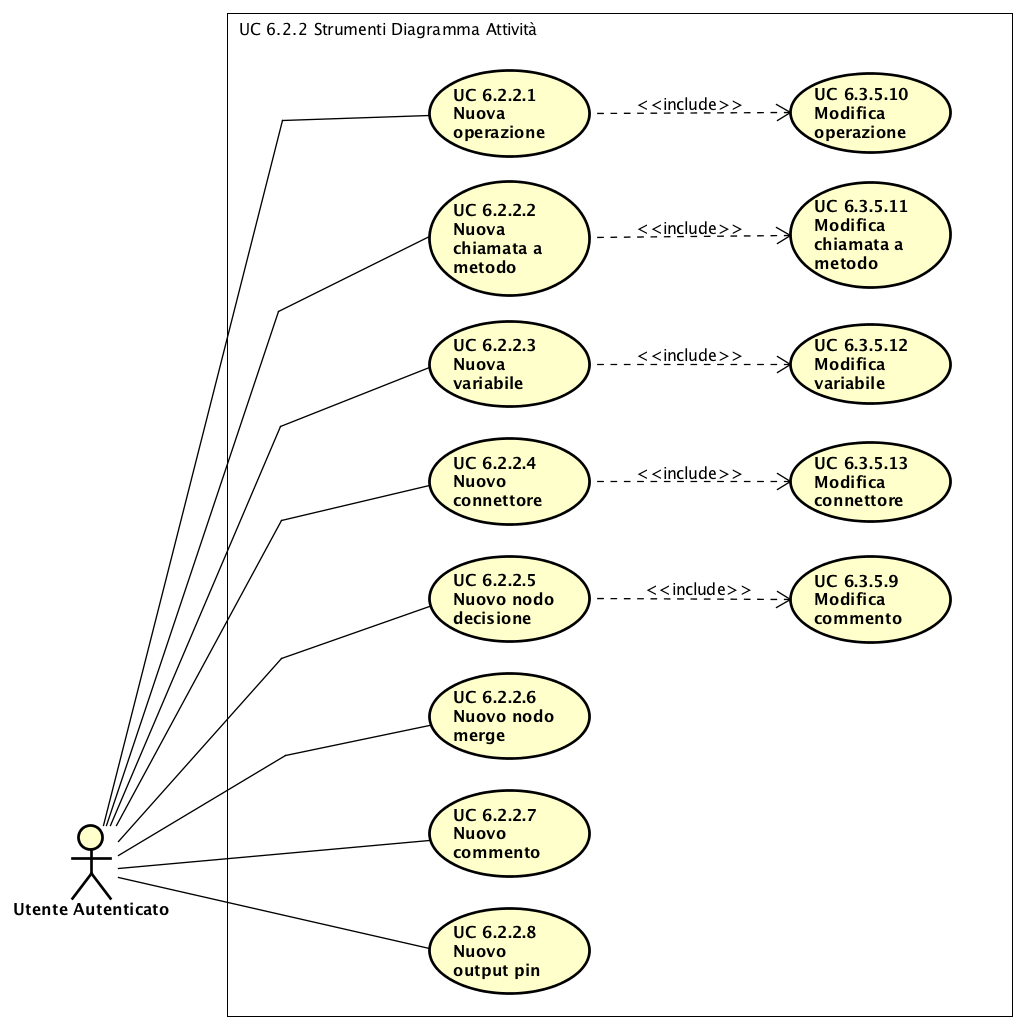
\includegraphics[scale=0.5]{../../Casi D'uso/UC6.2.2.png}
\caption{Caso d'uso UC6.2.2}
 \end{figure}
\begin{itemize}
\item \textbf{Attori}: \glossaryItem{Utente} autenticato;
\item \textbf{Descrizione}: L'attore può selezionare da questa lista uno degli strumenti per la creazione di \glossaryItem{Diagrammi delle attività};
\item \textbf{Precondizione}: L'attore deve aver caricato un progetto;
\item \textbf{Postcondizione}: L'\glossaryItem{Applicazione} visualizza la lista di strumenti necessari per il disegno di \glossaryItem{Diagrammi delle attività};
\item \textbf{Scenario principale}: \begin{enumerate}\item Nuova operazione (UC6.2.2.1);\item Nuova chiamata a \glossaryItem{Metodo} (UC6.2.2.2);\item Nuova variabile (UC6.2.2.3);\item Nuovo connettore (UC6.2.2.4);\item Nuovo nodo decisione (UC6.2.2.5);\item Nuovo nodo \glossaryItem{Merge} (UC6.2.2.6);\item Nuovo commento (UC6.2.2.7);\item Nuovo output pin (UC6.2.2.8);
 \end{enumerate}
 \item \textbf{Inclusioni}: \begin{itemize}
 \item \textbf{ Modifica operazione (UC 6.3.5.10)};
 \item \textbf{ Modifica chiamata a \glossaryItem{Metodo} (UC 6.3.5.11)};
 \item \textbf{ Modifica variabile (UC 6.3.5.12)};
  \item \textbf{ Modifica connettore (UC 6.3.5.13)};
  \item \textbf{ Modifica commento (UC 6.3.5.9)};
 \end{itemize}

\end{itemize}
\subsection{UC6.2.2.1 - Nuova operazione}
\label{ssec:UC6.2.2.1}
\begin{itemize}
\item \textbf{Attori}: \glossaryItem{Utente} autenticato;
\item \textbf{Descrizione}: L'attore può aggiungere un nuovo elemento operazione al \glossaryItem{Diagramma delle attività} di un \glossaryItem{Metodo};
\item \textbf{Precondizione}: Viene selezionato un \glossaryItem{Metodo} di una \glossaryItem{Classe} che risiede nel \glossaryItem{Frame} del \glossaryItem{Diagramma} delle  \glossaryItem{Classi};
\item \textbf{Postcondizione}: Viene aggiunto al \glossaryItem{Diagramma delle attività} di un \glossaryItem{Metodo} un nuovo elemento operazione;
\item \textbf{Scenario principale}: L'attore aggiunge un nuovo elemento operazione al diagramma delle attività;
\item \textbf{Scenari alternativi}: L'elemento non è posizionato all'interno della finestra del \glossaryItem{Diagramma delle attività} di un \glossaryItem{Metodo}.
\end{itemize}
\subsection{UC6.2.2.2 - Nuova chiamata a metodo}
\label{ssec:UC6.2.2.2}
\begin{itemize}
\item \textbf{Attori}: \glossaryItem{Utente} autenticato;
\item \textbf{Descrizione}: L'attore può aggiungere un elemento "chiamata a \glossaryItem{Metodo}" al \glossaryItem{Diagramma delle attività} di un \glossaryItem{Metodo};
\item \textbf{Precondizione}: Il \glossaryItem{Metodo} di una \glossaryItem{Classe} è stato selezionato ed è visualizzata correttamente la finestra del \glossaryItem{Diagramma delle attività} di esso;
\item \textbf{Postcondizione}: Un elemento chiamata a \glossaryItem{Metodo} è aggiunto al \glossaryItem{Diagramma delle attività} del \glossaryItem{Metodo} di una \glossaryItem{Classe};
\item \textbf{Scenario principale}: L'attore aggiunge un nuovo elemento chiamata a metodo al diagramma delle attività;
\item \textbf{Scenari alternativi}: L'elemento non è posizionato all'interno della finestra del \glossaryItem{Diagramma delle attività} di un \glossaryItem{Metodo}.
\end{itemize}
\subsection{UC6.2.2.3 - Nuova variabile}
\label{ssec:UC6.2.2.3}
\begin{itemize}
\item \textbf{Attori}: \glossaryItem{Utente} autenticato;
\item \textbf{Descrizione}: L'attore può aggiungere un nuovo elemento variabile al \glossaryItem{Diagramma delle attività} di un \glossaryItem{Metodo};
\item \textbf{Precondizione}: Viene selezionato un \glossaryItem{Metodo} di una \glossaryItem{Classe} che risiede nel \glossaryItem{Frame} del \glossaryItem{Diagramma} delle  \glossaryItem{Classi};
\item \textbf{Postcondizione}: Viene aggiunto al \glossaryItem{Diagramma delle attività} di un \glossaryItem{Metodo} un nuovo elemento variabile;
\item \textbf{Scenario principale}: L'attore aggiunge un nuovo elemento variabile al diagramma delle attività.
\end{itemize}
\subsection{UC6.2.2.4 - Nuovo connettore}
\label{ssec:UC6.2.2.4}
\begin{itemize}
\item \textbf{Attori}: \glossaryItem{Utente} autenticato;
\item \textbf{Descrizione}: L'attore può aggiungere un nuovo elemento connettore al \glossaryItem{Diagramma delle attività} di un \glossaryItem{Metodo};
\item \textbf{Precondizione}: Viene selezionato un \glossaryItem{Metodo} di una \glossaryItem{Classe} che risiede nel \glossaryItem{Frame} del \glossaryItem{Diagramma} delle  \glossaryItem{Classi}; Devono esserci nel \glossaryItem{Diagramma delle attività} del \glossaryItem{Metodo} almeno due elementi che possono essere connessi;
\item \textbf{Postcondizione}: Viene aggiunto al \glossaryItem{Diagramma delle attività} di un \glossaryItem{Metodo} un nuovo elemento connettore;
\item \textbf{Scenari alternativi}: L'elemento non è posizionato all'interno della finestra del \glossaryItem{Diagramma delle attività} di un \glossaryItem{Metodo};
\item \textbf{Scenario principale}: L'attore aggiunge un nuovo elemento connettore al diagramma delle attività.
\end{itemize}
\subsection{UC6.2.2.5 - Nuovo nodo decisione}
\label{ssec:UC6.2.2.5}
\begin{itemize}
\item \textbf{Attori}: \glossaryItem{Utente} autenticato;
\item \textbf{Descrizione}: L'attore può aggiungere un nuovo elemento nodo decisione al \glossaryItem{Diagramma delle attività} di un \glossaryItem{Metodo};
\item \textbf{Precondizione}: Viene selezionato un \glossaryItem{Metodo} di una \glossaryItem{Classe} che risiede nel \glossaryItem{Frame} del \glossaryItem{Diagramma} delle  \glossaryItem{Classi};
\item \textbf{Postcondizione}: Viene aggiunto al \glossaryItem{Diagramma delle attività} di un \glossaryItem{Metodo} un nuovo elemento nodo decisione;
\item \textbf{Scenario principale}: L'attore aggiunge un nuovo elemento nodo di decisione al diagramma delle attività.
\end{itemize}
\subsection{UC6.2.2.6 - Nuovo nodo merge}
\label{ssec:UC6.2.2.6}
\begin{itemize}
\item \textbf{Attori}: \glossaryItem{Utente} autenticato;
\item \textbf{Descrizione}: L'attore può aggiungere un nuovo elemento nodo \glossaryItem{Merge} al \glossaryItem{Diagramma delle attività} di un \glossaryItem{Metodo};
\item \textbf{Precondizione}: Viene selezionato un \glossaryItem{Metodo} di una \glossaryItem{Classe} che risiede nel \glossaryItem{Frame} del \glossaryItem{Diagramma} delle  \glossaryItem{Classi};
\item \textbf{Postcondizione}: Viene aggiunto al \glossaryItem{Diagramma delle attività} di un \glossaryItem{Metodo} un nuovo elemento nodo \glossaryItem{Merge};
\item \textbf{Scenario principale}: L'attore aggiunge un nuovo elemento merge al diagramma delle attività;.
\end{itemize}
\subsection{UC6.2.2.7 - Nuovo commento}
\label{ssec:UC6.2.2.7}
\begin{itemize}
\item \textbf{Attori}: \glossaryItem{Utente} autenticato;
\item \textbf{Descrizione}: L'attore può aggiungere un nuovo elemento commento al \glossaryItem{Diagramma delle attività} di un \glossaryItem{Metodo};
\item \textbf{Precondizione}: Viene selezionato un \glossaryItem{Metodo} di una \glossaryItem{Classe} che risiede nel \glossaryItem{Frame} del \glossaryItem{Diagramma} delle  \glossaryItem{Classi};
\item \textbf{Postcondizione}: Viene aggiunto al \glossaryItem{Diagramma delle attività} di un \glossaryItem{Metodo} un nuovo elemento commento;
\item \textbf{Scenario principale}: L'attore aggiunge un nuovo elemento commento al diagramma delle attività;
\end{itemize}
\subsection{UC6.2.2.8 - Nuovo output pin}
\label{ssec:UC6.2.2.8}
\begin{itemize}
\item \textbf{Attori}: \glossaryItem{Utente} autenticato;
\item \textbf{Descrizione}: L'attore può annettere un nuovo output pin ad un elemento chiamata a \glossaryItem{Metodo}, presente nel \glossaryItem{Diagramma delle attività} di un \glossaryItem{Metodo};
\item \textbf{Precondizione}: Viene selezionato un \glossaryItem{Metodo} di una \glossaryItem{Classe} che risiede nel \glossaryItem{Frame} del \glossaryItem{Diagramma} delle  \glossaryItem{Classi}; è presente un elemento chiamata a \glossaryItem{Metodo} nel \glossaryItem{Diagramma};
\item \textbf{Postcondizione}: Viene annesso ad un elemento chiamata a \glossaryItem{Metodo}, presente nel \glossaryItem{Diagramma delle attività} di un \glossaryItem{Metodo}, un nuovo elemento output pin;
\item \textbf{Scenario principale}: L'attore aggiunge un nuovo elemento output pin al diagramma delle attività.
\end{itemize}
\newpage
\subsection{UC6.3 - Disegnatore diagrammi}
\label{ssec:UC6.3}
\begin{figure}[h!]
\centering
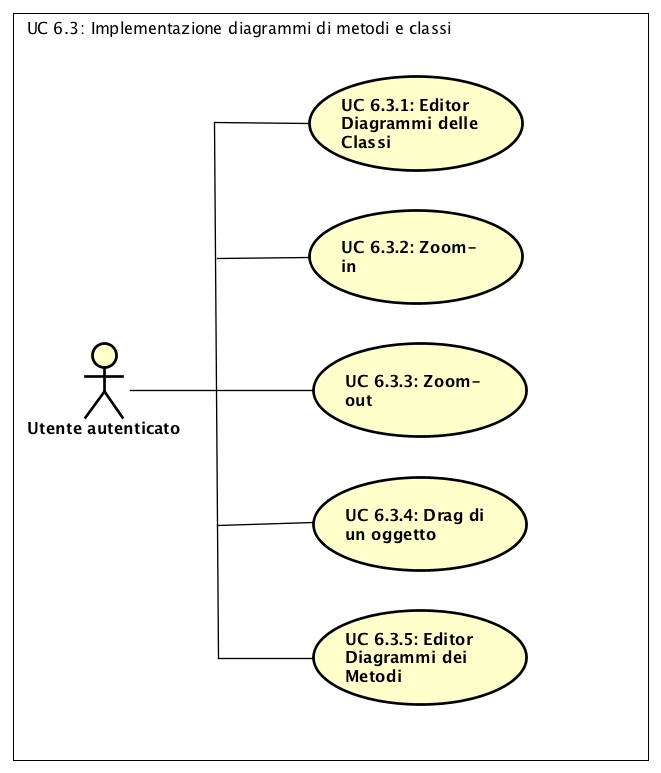
\includegraphics[scale=0.5]{../../Casi D'uso/UC6.3.png}
\caption{Caso d'uso UC6.3}
 \end{figure}
\begin{itemize}
\item \textbf{Attori}: \glossaryItem{Utente} autenticato;
\item \textbf{Descrizione}: L'attore può implementare programmi disegnando \glossaryItem{Diagrammi};
\item \textbf{Precondizione}: L'\glossaryItem{Applicazione} rende disponibile il \glossaryItem{Frame} di disegno;
\item \textbf{Postcondizione}: L'\glossaryItem{Applicazione} disegna i \glossaryItem{Diagrammi} richiesti dall'attore;
\item \textbf{Scenario principale}: \begin{enumerate}\item Editor \glossaryItem{Diagrammi} delle \glossaryItem{Classi} (UC6.3.1);\item \glossaryItem{Zoom}-in (UC6.3.2);\item \glossaryItem{Zoom}-out (UC6.3.3);\item Drag di un oggetto (UC6.3.4);\item Editor \glossaryItem{Diagrammi} dei \glossaryItem{Metodi} (UC6.3.5).
 \end{enumerate}
\end{itemize}
\newpage
\subsection{UC6.3.1 - Editor \glossaryItem{Diagrammi delle classi}}
\label{ssec:UC6.3.1}
\begin{figure}[h!]
\centering
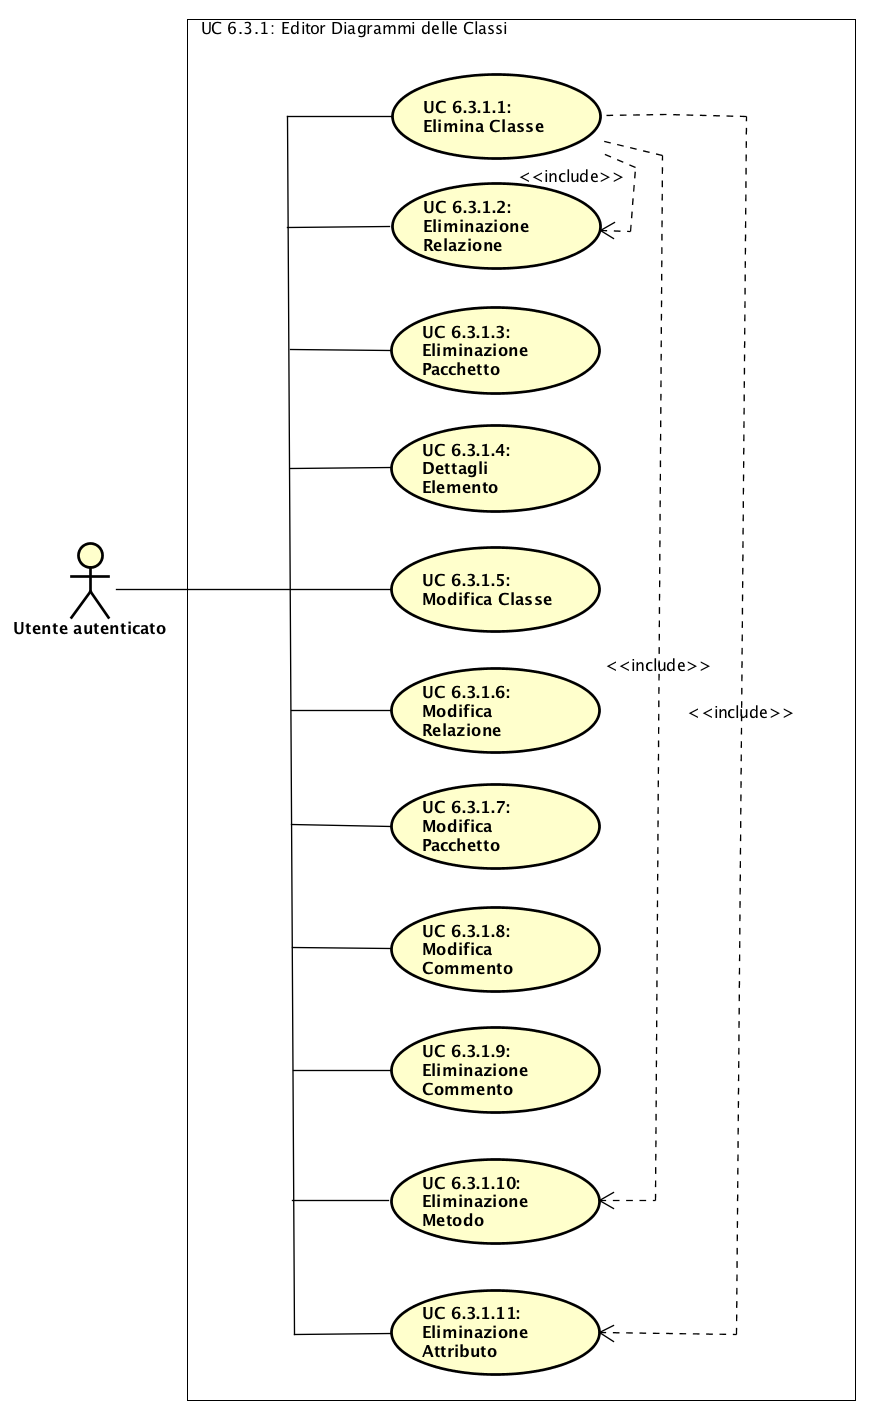
\includegraphics[scale=0.5]{../../Casi D'uso/UC6.3.1.png}
\caption{Caso d'uso UC6.3.1}
 \end{figure}
\begin{itemize}
\item \textbf{Attori}: \glossaryItem{Utente} autenticato;
\item \textbf{Descrizione}: L'attore può interagire con la schermata principale;
\item \textbf{Precondizione}: L'attore crea o apre un progetto;
\item \textbf{Postcondizione}: L'attore chiude il progetto;
\item \textbf{Scenario principale}: \begin{enumerate}\item Eliminazione \glossaryItem{Classe} (UC6.3.1.1);\item Eliminazione Relazione (UC6.3.1.2);\item Eliminazione pacchetto (UC6.3.1.3);\item Dettagli Elemento (UC6.3.1.4);\item Modifica \glossaryItem{Classe} (UC6.3.1.5);\item Modifica Relazione (UC6.3.1.6);\item Modifica pacchetto (UC6.3.1.7);\item Modifica commento (UC6.3.1.8);\item Eliminazione commento (UC6.3.1.9).
 \end{enumerate}
\end{itemize}
\subsection{UC6.3.1.1 - Eliminazione Classe}
\label{ssec:UC6.3.1.1}
\begin{figure}[h!]
\centering
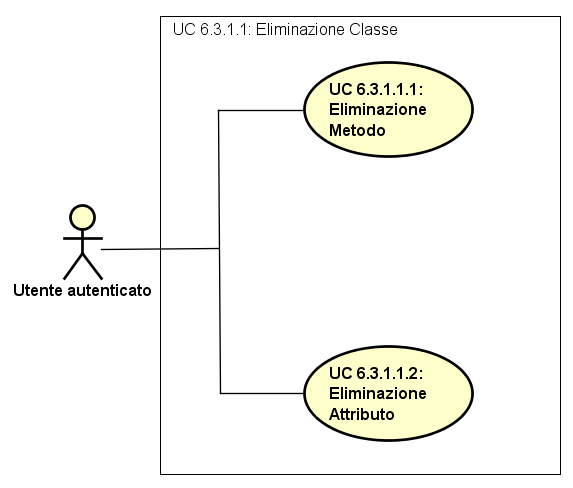
\includegraphics[scale=0.5]{../../Casi D'uso/UC6.3.1.1.png}
\caption{Caso d'uso UC6.3.1.1}
 \end{figure}
\begin{itemize}
\item \textbf{Attori}: \glossaryItem{Utente} autenticato;
\item \textbf{Descrizione}: L'attore può eliminare una \glossaryItem{Classe} dal progetto corrente;
\item \textbf{Precondizione}: Deve essere stata disegnata una \glossaryItem{Classe};
\item \textbf{Postcondizione}: Viene eliminata la \glossaryItem{Classe} selezionata e, a cascata, tutti i \glossaryItem{Metodi} ad essa, e solo ad essa, associati, tutti gli attributi e tutte le relazioni che la coinvolgono;
\item \textbf{Scenario principale}: \begin{enumerate}\item Eliminazione \glossaryItem{Metodo} (UC6.3.1.1.1);\item Eliminazione Attributo (UC6.3.1.1.2).
 \end{enumerate}
\end{itemize}
\subsection{UC6.3.1.1.1 - Eliminazione Metodo}
\label{ssec:UC6.3.1.1.1}
\begin{itemize}
\item \textbf{Attori}: \glossaryItem{Utente} autenticato;
\item \textbf{Descrizione}: L'attore ha disegnato una \glossaryItem{Classe} con almeno un \glossaryItem{Metodo} ed  eventualmente anche il \glossaryItem{Diagramma delle attività} corrispondente e può eliminarlo;
\item \textbf{Precondizione}: È stata creata una \glossaryItem{Classe} con almeno un \glossaryItem{Metodo};
\item \textbf{Postcondizione}: Viene eliminato il \glossaryItem{Metodo} selezionato e, a cascata, il \glossaryItem{Diagramma delle attività} associato se esistente;
\item \textbf{Scenario principale}: L'attore elimina un metodo di una classe;
\item \textbf{Scenari alternativi}: L'attore ha aggiunto un nuovo \glossaryItem{Metodo} e desidera eliminarlo.
\end{itemize}
\subsection{UC6.3.1.1.2 - Eliminazione Attributo}
\label{ssec:UC6.3.1.1.2}
\begin{itemize}
\item \textbf{Attori}: \glossaryItem{Utente} autenticato;
\item \textbf{Descrizione}: L'attore ha disegnato una \glossaryItem{Classe} con almeno un attributo al suo interno e può eliminarlo;
\item \textbf{Precondizione}: È stata creata una \glossaryItem{Classe} con almeno un attributo;
\item \textbf{Postcondizione}: L'attributo selezionato viene eliminato;
\item \textbf{Scenario principale}: L'attore elimina un attributo di una classe;
\item \textbf{Scenari alternativi}: L'attore ha aggiunto un nuovo attributo e desidera eliminarlo.
\end{itemize}
\subsection{UC6.3.1.2 - Eliminazione Relazione}
\label{ssec:UC6.3.1.2}
\begin{itemize}
\item \textbf{Attori}: \glossaryItem{Utente} autenticato;
\item \textbf{Descrizione}: L'attore può eliminare una relazione fra oggetti all'interno del \glossaryItem{Designer};
\item \textbf{Precondizione}: È stata disegnata una relazione;
\item \textbf{Postcondizione}: Viene eliminata la relazione selezionata ed eventuali etichette associate;
\item \textbf{Scenario principale}: L'attore elimina una relazione tra classi.
\end{itemize}
\subsection{UC6.3.1.3 - Eliminazione pacchetto}
\label{ssec:UC6.3.1.3}
\begin{itemize}
\item \textbf{Attori}: \glossaryItem{Utente} autenticato;
\item \textbf{Descrizione}: L'attore può eliminare un pacchetto;
\item \textbf{Precondizione}: È stato disegnato un pacchetto;
\item \textbf{Postcondizione}: Viene eliminato il pacchetto dal \glossaryItem{Designer} assieme a tutti i suoi eventuali elementi contenuti;
\item \textbf{Scenario principale}: L'attore elimina un package.
\end{itemize}
\subsection{UC6.3.1.4 - Dettagli Elemento}
\label{ssec:UC6.3.1.4}
\begin{itemize}
\item \textbf{Attori}: \glossaryItem{Utente} autenticato;
\item \textbf{Descrizione}: L'attore può visualizzare i dettagli implementativi dell'elemento desiderato;
\item \textbf{Precondizione}: È stato disegnato almeno un elemento all'interno del \glossaryItem{Designer};
\item \textbf{Postcondizione}: Vengono visualizzati tutti i dettagli dell'elemento;
\item \textbf{Scenario principale}: L'attore visualizza i dettagli implementativi dell'elemento selezionato.
\end{itemize}
\newpage
\subsection{UC6.3.1.5 - Modifica Classe}
\label{ssec:UC6.3.1.5}
\begin{figure}[h!]
\centering
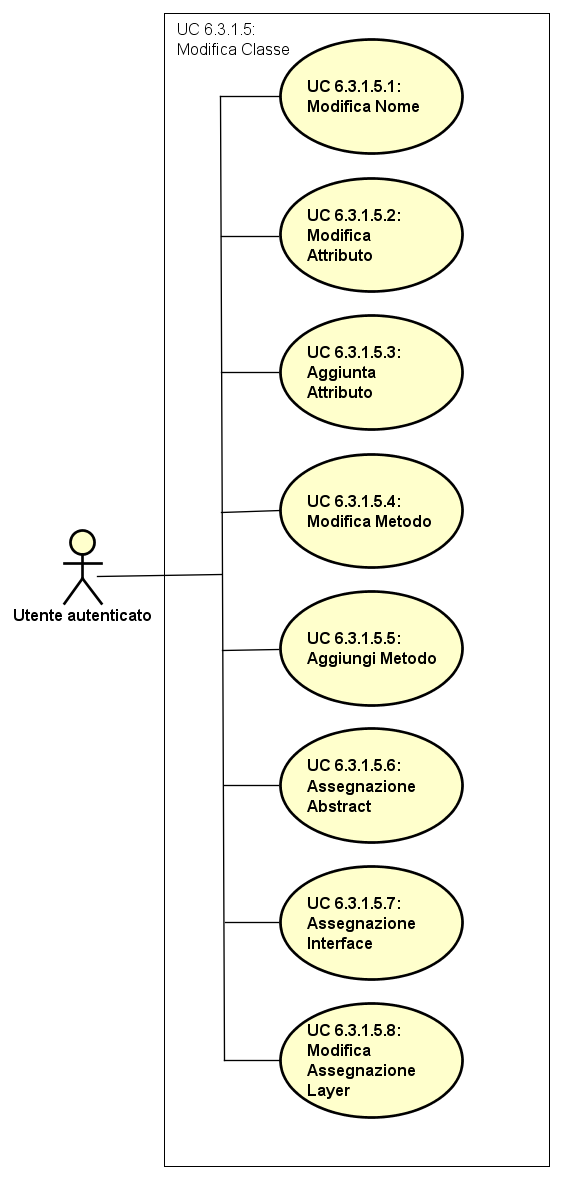
\includegraphics[scale=0.5]{../../Casi D'uso/UC6.3.1.5.png}
\caption{Caso d'uso UC6.3.1.5}
 \end{figure}
\begin{itemize}
\item \textbf{Attori}: \glossaryItem{Utente} autenticato;
\item \textbf{Descrizione}: L'attore può modificare degli elementi interni ad una \glossaryItem{Classe};
\item \textbf{Precondizione}: È stata disegnata una \glossaryItem{Classe} sul progetto;
\item \textbf{Postcondizione}: La \glossaryItem{Classe} risulta modificata;
\item \textbf{Scenario principale}: \begin{enumerate}\item Modifica Nome (UC6.3.1.5.1);\item Modifica Attributo (UC6.3.1.5.2);\item Aggiunta attributo (UC6.3.1.5.3);\item Modifica \glossaryItem{Metodo} (UC6.3.1.5.4);\item Aggiungi \glossaryItem{Metodo} (UC6.3.1.5.5);\item Assegnazione Abstract (UC6.3.1.5.6);\item Assegnazione interface (UC6.3.1.5.7);\item Modifica assegnazione layer (UC6.3.1.5.8).
 \end{enumerate}
\end{itemize}
\subsection{UC6.3.1.5.1 - Modifica Nome}
\label{ssec:UC6.3.1.5.1}
\begin{itemize}
\item \textbf{Attori}: \glossaryItem{Utente} autenticato;
\item \textbf{Descrizione}: L'attore può modificare il nome della \glossaryItem{Classe};
\item \textbf{Precondizione}: È stata creata una \glossaryItem{Classe} con un nome;
\item \textbf{Postcondizione}: Viene modificato il nome della \glossaryItem{Classe};
\item \textbf{Scenario principale}: L'attore modifica il nome di una classe.
\end{itemize}
\subsection{UC6.3.1.5.2 - Modifica Attributo}
\label{ssec:UC6.3.1.5.2}
\begin{figure}[h!]
\centering
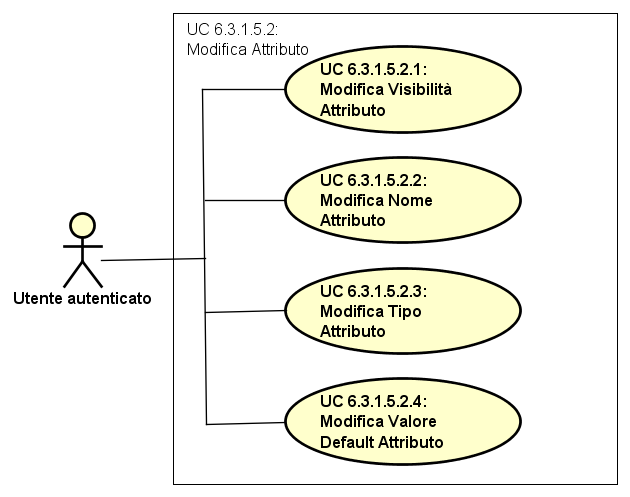
\includegraphics[scale=0.5]{../../Casi D'uso/UC6.3.1.5.2.png}
\caption{Caso d'uso UC6.3.1.5.2}
 \end{figure}
\begin{itemize}
\item \textbf{Attori}: \glossaryItem{Utente} autenticato;
\item \textbf{Descrizione}: L'attore può modificare l'attributo della \glossaryItem{Classe};
\item \textbf{Precondizione}: È stata disegnata una \glossaryItem{Classe} con almeno un attributo;
\item \textbf{Postcondizione}: Viene modificato l'attributo selezionato;
\item \textbf{Scenario principale}: \begin{enumerate}\item Modifica visibilità attributo (UC6.3.1.5.2.1);\item Modifica nome attributo (UC6.3.1.5.2.2);\item Modifica tipo attributo (UC6.3.1.5.2.3);\item Modifica valore default attributo (UC6.3.1.5.2.4).
 \end{enumerate}
\end{itemize}
\subsection{UC6.3.1.5.2.1 - Modifica visibilità attributo}
\label{ssec:UC6.3.1.5.2.1}
\begin{itemize}
\item \textbf{Attori}: \glossaryItem{Utente} autenticato;
\item \textbf{Descrizione}: L'attore può scegliere la visibilità per l'attributo;
\item \textbf{Precondizione}: Viene visualizzato un form che permette la selezione della visibilità;
\item \textbf{Postcondizione}: L'\glossaryItem{Applicazione} registra il dato inserito;
\item \textbf{Scenario principale}: L'attore modifica la visibilità di un attributo.
\end{itemize}
\subsection{UC6.3.1.5.2.2 - Modifica nome attributo}
\label{ssec:UC6.3.1.5.2.2}
\begin{itemize}
\item \textbf{Attori}: \glossaryItem{Utente} autenticato;
\item \textbf{Descrizione}: L'attore può inserire il nome per l'attributo;
\item \textbf{Precondizione}: Viene visualizzato un form che permette l'inserimento del nome dell'attributo;
\item \textbf{Postcondizione}: L'\glossaryItem{Applicazione} registra il dato inserito;
\item \textbf{Scenario principale}: L'attore modifica il nome di un attributo.
\end{itemize}
\subsection{UC6.3.1.5.2.3 - Modifica tipo attributo}
\label{ssec:UC6.3.1.5.2.3}
\begin{itemize}
\item \textbf{Attori}: \glossaryItem{Utente} autenticato;
\item \textbf{Descrizione}: L'attore può inserire il tipo dell'attributo che si sta inserendo;
\item \textbf{Precondizione}: Viene visualizzato un form che permette l'inserimento tipo dell'attributo;
\item \textbf{Postcondizione}: L'\glossaryItem{Applicazione} registra il dato inserito;
\item \textbf{Scenario principale}: L'attore modifica il tipo di un attributo.
\end{itemize}
\subsection{UC6.3.1.5.2.4 - Modifica valore default attributo}
\label{ssec:UC6.3.1.5.2.4}
\begin{itemize}
\item \textbf{Attori}: \glossaryItem{Utente} autenticato;
\item \textbf{Descrizione}: L'attore può inserire il valore di default che può avere l'attributo;
\item \textbf{Precondizione}: Viene visualizzato un form che permette l'inserimento del valore di default dell'attributo;
\item \textbf{Postcondizione}: L'\glossaryItem{Applicazione} registra il dato inserito;
\item \textbf{Scenario principale}: L'attore modifica il valore di default di un attributo.
\end{itemize}
\subsection{UC6.3.1.5.3 - Aggiunta attributo}
\label{ssec:UC6.3.1.5.3}
\begin{itemize}
\item \textbf{Attori}: \glossaryItem{Utente} autenticato;
\item \textbf{Descrizione}: L'attore può inserire un attributo per la \glossaryItem{Classe} selezionata;
\item \textbf{Precondizione}: Viene visualizzato un form che permette l'inserimento di attributi della \glossaryItem{Classe};
\item \textbf{Postcondizione}: L'\glossaryItem{Applicazione} registra il dato inserito;
\item \textbf{Scenario principale}: L'attore inserisce un nuovo attributo.
\end{itemize}
\subsection{UC6.3.1.5.4 - Modifica Metodo}
\label{ssec:UC6.3.1.5.4}
\begin{figure}[h!]
\centering
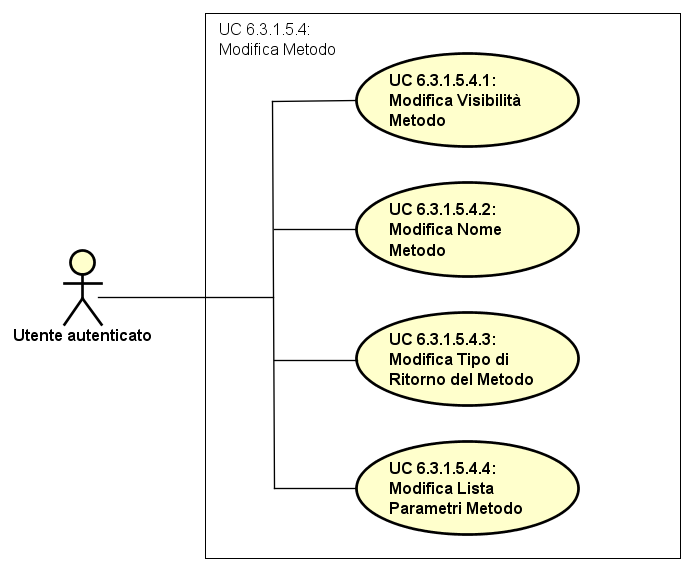
\includegraphics[scale=0.5]{../../Casi D'uso/UC6.3.1.5.4.png}
\caption{Caso d'uso UC6.3.1.5.4}
 \end{figure}
\begin{itemize}
\item \textbf{Attori}: \glossaryItem{Utente} autenticato;
\item \textbf{Descrizione}: L'attore può modificare il \glossaryItem{Metodo} della \glossaryItem{Classe};
\item \textbf{Precondizione}: È stata creata una \glossaryItem{Classe} con almeno un \glossaryItem{Metodo} al suo interno;
\item \textbf{Postcondizione}: Il \glossaryItem{Metodo} selezionato viene modificato;
\item \textbf{Scenario principale}: \begin{enumerate}\item Modifica visibilità \glossaryItem{Metodo} (UC6.3.1.5.4.1);\item Modifica nome \glossaryItem{Metodo} (UC6.3.1.5.4.2);\item Modifica tipo di ritorno del \glossaryItem{Metodo} (UC6.3.1.5.4.3);\item Modifica lista parametri \glossaryItem{Metodo} (UC6.3.1.5.4.4).
 \end{enumerate}
\end{itemize}
\subsection{UC6.3.1.5.4.1 - Modifica visibilità metodo}
\label{ssec:UC6.3.1.5.4.1}
\begin{itemize}
\item \textbf{Attori}: \glossaryItem{Utente} autenticato;
\item \textbf{Descrizione}: L'attore può scegliere la visibilità per un \glossaryItem{Metodo};
\item \textbf{Precondizione}: Viene visualizzato un form che permette la selezione della visibilità;
\item \textbf{Postcondizione}: L'\glossaryItem{Applicazione} registra il dato inserito;
\item \textbf{Scenario principale}: L'attore modifica la visibilità di un metodo.
\end{itemize}
\subsection{UC6.3.1.5.4.2 - Modifica nome metodo}
\label{ssec:UC6.3.1.5.4.2}
\begin{itemize}
\item \textbf{Attori}: \glossaryItem{Utente} autenticato;
\item \textbf{Descrizione}: L'attore può inserire il nome per il \glossaryItem{Metodo};
\item \textbf{Precondizione}: Viene visualizzato un form che permette l'inserimento del nome del \glossaryItem{Metodo};
\item \textbf{Postcondizione}: L'\glossaryItem{Applicazione} registra il dato inserito;
\item \textbf{Scenario principale}: L'attore modifica il nome di un metodo.
\end{itemize}
\subsection{UC6.3.1.5.4.3 - Modifica tipo di ritorno del metodo}
\label{ssec:UC6.3.1.5.4.3}
\begin{itemize}
\item \textbf{Attori}: \glossaryItem{Utente} autenticato;
\item \textbf{Descrizione}: L'attore può inserire il tipo di ritorno per il \glossaryItem{Metodo};
\item \textbf{Precondizione}: Viene visualizzato un form che permette l'inserimento tipo di ritorno del \glossaryItem{Metodo};
\item \textbf{Postcondizione}: L'\glossaryItem{Applicazione} registra il dato inserito;
\item \textbf{Scenario principale}: L'attore modifica il tipo di ritorno di un metodo.
\end{itemize}
\subsection{UC6.3.1.5.4.4 - Modifica lista parametri metodo}
\label{ssec:UC6.3.1.5.4.4}
\begin{itemize}
\item \textbf{Attori}: \glossaryItem{Utente} autenticato;
\item \textbf{Descrizione}: L'attore può inserire la lista dei parametri che verranno utilizzati nella realizzazione del \glossaryItem{Metodo};
\item \textbf{Precondizione}: Viene visualizzato un form che permette l'inserimento della lista dei parametri;
\item \textbf{Postcondizione}: L'\glossaryItem{Applicazione} registra il dato inserito;
\item \textbf{Scenario principale}: L'attore modifica la lista di parametri di un metodo.
\end{itemize}
\subsection{UC6.3.1.5.5 - Aggiungi Metodo}
\label{ssec:UC6.3.1.5.5}
\begin{itemize}
\item \textbf{Attori}: \glossaryItem{Utente} autenticato;
\item \textbf{Descrizione}: L'attore può aggiungere un \glossaryItem{Metodo};
\item \textbf{Precondizione}: Deve essere presente la \glossaryItem{Classe} alla quale si vuole aggiungere il \glossaryItem{Metodo};
\item \textbf{Postcondizione}: Il \glossaryItem{Metodo} viene aggiunto alla \glossaryItem{Classe} prescelta;
\item \textbf{Scenario principale}: L'attore aggiunge un nuovo metodo.
\end{itemize}
\subsection{UC6.3.1.5.6 - Assegnazione Abstract}
\label{ssec:UC6.3.1.5.6}
\begin{itemize}
\item \textbf{Attori}: \glossaryItem{Utente} autenticato;
\item \textbf{Descrizione}: L'attore definisce se la \glossaryItem{Classe} è astratta;
\item \textbf{Precondizione}: Viene visualizzato un form che permette l'assegnazione della keyword <<abstract>>;
\item \textbf{Postcondizione}: L'\glossaryItem{Applicazione} registra il dato inserito;
\item \textbf{Scenario principale}: L'attore assegna il valore abstract in una classe.
\end{itemize}
\subsection{UC6.3.1.5.7 - Assegnazione interface}
\label{ssec:UC6.3.1.5.7}
\begin{itemize}
\item \textbf{Attori}: \glossaryItem{Utente} autenticato;
\item \textbf{Descrizione}: L'attore definisce se la \glossaryItem{Classe} un'interfaccia;
\item \textbf{Precondizione}: Viene visualizzato un form che permette l'assegnazione della keyword <<interface>>;
\item \textbf{Postcondizione}: L'\glossaryItem{Applicazione} registra il dato inserito;
\item \textbf{Scenario principale}: L'attore assegna il valore interface in una classe.
\end{itemize}
\subsection{UC6.3.1.5.8 - Modifica assegnazione layer}
\label{ssec:UC6.3.1.5.8}
\begin{itemize}
\item \textbf{Attori}: \glossaryItem{Utente} autenticato;
\item \textbf{Descrizione}: L'attore può selezionare il layer a cui vuole associare la \glossaryItem{Classe};
\item \textbf{Precondizione}: Viene visualizzato un form che permette l'assegnazione del layer;
\item \textbf{Postcondizione}: L'\glossaryItem{Applicazione} registra il dato inserito;
\item \textbf{Scenario principale}: L'attore modifica l'assegnazione ad un layer di una classe.
\end{itemize}
\subsection{UC6.3.1.6 - Modifica Relazione}
\label{ssec:UC6.3.1.6}
\begin{itemize}
\item \textbf{Attori}: \glossaryItem{Utente} autenticato;
\item \textbf{Descrizione}: L'attore può modificare l'etichetta della relazione;
\item \textbf{Precondizione}: È stata creata una relazione fra due o più \glossaryItem{Classi};
\item \textbf{Postcondizione}: L'etichetta della relazione corrente è stata modificata;
\item \textbf{Scenario principale}: L'attore modifica l'etichetta di una relazione.
\end{itemize}
\subsection{UC6.3.1.7 - Modifica pacchetto}
\label{ssec:UC6.3.1.7}
\begin{figure}[h!]
\centering
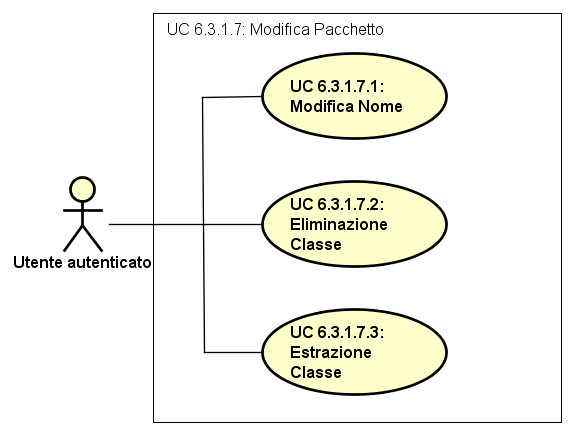
\includegraphics[scale=0.5]{../../Casi D'uso/UC6.3.1.7.png}
\caption{Caso d'uso UC6.3.1.7}
 \end{figure}
\begin{itemize}
\item \textbf{Attori}: \glossaryItem{Utente} autenticato;
\item \textbf{Descrizione}: L'attore può modificare un pacchetto;
\item \textbf{Precondizione}: È stato creato un pacchetto;
\item \textbf{Postcondizione}: Il pacchetto è stato modificato;
\item \textbf{Scenario principale}: \begin{enumerate}\item Modifica Nome (UC6.3.1.7.1);\item Eliminazione \glossaryItem{Classe} (UC6.3.1.7.2);\item Estrazione \glossaryItem{Classe} (UC6.3.1.7.3).
 \end{enumerate}
\end{itemize}
\subsection{UC6.3.1.7.1 - Modifica Nome}
\label{ssec:UC6.3.1.7.1}
\begin{itemize}
\item \textbf{Attori}: \glossaryItem{Utente} autenticato.
\item \textbf{Descrizione}: L'attore può modificare il nome di un pacchetto, tale nome deve essere univoco;
\item \textbf{Precondizione}: È stato creato un pacchetto e viene visualizzato un form che permette l'inserimento del nome;
\item \textbf{Postcondizione}: Il nome del pacchetto selezionato viene salvato;
\item \textbf{Scenario principale}: L'attore modifica il nome di un pacchetto.
\end{itemize}
\subsection{UC6.3.1.7.2 - Eliminazione classe}
\label{ssec:UC6.3.1.7.2}
\begin{itemize}
\item \textbf{Attori}: \glossaryItem{Utente} autenticato;
\item \textbf{Descrizione}: L'attore può eliminare una \glossaryItem{Classe} all'interno del pacchetto;
\item \textbf{Precondizione}: Esiste un pacchetto con almeno una \glossaryItem{Classe} al suo interno;
\item \textbf{Postcondizione}: La \glossaryItem{Classe} selezionata viene eliminata dal pacchetto;
\item \textbf{Scenario principale}: L'attore elimina una classe in un pacchetto.
\end{itemize}
\subsection{UC6.3.1.7.3 - Estrazione classe}
\label{ssec:UC6.3.1.7.3}
\begin{itemize}
\item \textbf{Attori}: \glossaryItem{Utente} autenticato;
\item \textbf{Descrizione}: L'attore può estrarre una \glossaryItem{Classe} dal pacchetto;
\item \textbf{Precondizione}: Esiste un pacchetto con almeno una \glossaryItem{Classe} al suo interno;
\item \textbf{Postcondizione}: La \glossaryItem{Classe} selezionata si trova fuori dal pacchetto;
\item \textbf{Scenario principale}: L'attore estra una classe in un pacchetto.
\end{itemize}
\subsection{UC6.3.1.8 - Modifica commento}
\label{ssec:UC6.3.1.8}
\begin{itemize}
\item \textbf{Attori}: \glossaryItem{Utente} autenticato;
\item \textbf{Descrizione}: L'attore può modificare il testo inserito nel commento;
\item \textbf{Precondizione}: E' stato inserito un commento;
\item \textbf{Postcondizione}: Il commento risulta modificato;
\item \textbf{Scenario principale}: \begin{enumerate}\item Modifica testo commento (UC6.3.1.8.1).
 \end{enumerate}
\end{itemize}
\subsection{UC6.3.1.8.1 - Modifica testo commento}
\label{ssec:UC6.3.1.8.1}
\begin{itemize}
\item \textbf{Attori}: \glossaryItem{Utente} autenticato;
\item \textbf{Descrizione}: L'attore può modificare il testo di un commento;
\item \textbf{Precondizione}: L'\glossaryItem{Applicazione} visualizza il form per l'inserimento dei dati;
\item \textbf{Postcondizione}: L'\glossaryItem{Applicazione} ha registrato il dato inserito;
\item \textbf{Scenario principale}: L'attore modifica il testo di un commento.
\end{itemize}
\subsection{UC6.3.1.9 - Eliminazione commento}
\label{ssec:UC6.3.1.9}
\begin{itemize}
\item \textbf{Attori}: \glossaryItem{Utente} autenticato;
\item \textbf{Descrizione}: L'attore può eliminare un commento del \glossaryItem{Diagramma} delle \glossaryItem{Classi};
\item \textbf{Precondizione}: È stato creato un \glossaryItem{Diagramma} delle \glossaryItem{Classi} con almeno un commento al suo interno;
\item \textbf{Postcondizione}: Il commento selezionato è stato eliminato;
\item \textbf{Scenario principale}: L'attore elimina un commento.
\end{itemize}
\subsection{UC6.3.2 - \glossaryItem{Zoom}-in}
\label{ssec:UC6.3.2}
\begin{itemize}
\item \textbf{Attori}: \glossaryItem{Utente} Autenticato.
\item \textbf{Descrizione}: L'attore può applicare lo \glossaryItem{Zoom}-in su una particolare zona del \glossaryItem{Designer};
\item \textbf{Precondizione}: È stato aperto o avviato un nuovo progetto e lo \glossaryItem{Zoom} non è ancora al massimo;
\item \textbf{Postcondizione}: Si è effettuato uno \glossaryItem{Zoom} nel punto indicato dal mouse;
\item \textbf{Scenario principale}: L'attore effettua lo Zoom-in in una particolare zona del designer.
\end{itemize}
\subsection{UC6.3.3 - \glossaryItem{Zoom}-out}
\label{ssec:UC6.3.3}
\begin{itemize}
\item \textbf{Attori}: \glossaryItem{Utente} autenticato;
\item \textbf{Descrizione}: L'attore può applicare lo \glossaryItem{Zoom}-out su una porzione del \glossaryItem{Designer};
\item \textbf{Precondizione}: È stato aperto o avviato un nuovo progetto ed è già stato operato almeno uno \glossaryItem{Zoom}-in;
\item \textbf{Postcondizione}: Viene effettuato uno \glossaryItem{Zoom}-out sulla porzione di \glossaryItem{Designer} desiderata;
\item \textbf{Scenario principale}: L'attore effettua lo Zoom-out in una particolare zona del designer.
\end{itemize}
\subsection{UC6.3.4 - Drag di un oggetto}
\label{ssec:UC6.3.4}
\begin{itemize}
\item \textbf{Attori}: \glossaryItem{Utente} autenticato;
\item \textbf{Descrizione}: L'attore può spostare un oggetto all'interno del \glossaryItem{Designer};
\item \textbf{Precondizione}: È stato disegnato almeno un oggetto, di qualsiasi natura, sul \glossaryItem{Designer};
\item \textbf{Postcondizione}: L'oggetto selezionato viene spostato nella posizione desiderata;
\item \textbf{Scenario principale}: L'attore effettua il Drag di un oggetto all'interno del designer.
\end{itemize}
\newpage
\subsection{UC6.3.5 - Editor \glossaryItem{Diagrammi} dei Metodi}
\label{ssec:UC6.3.5}
\begin{figure}[h!]
\centering
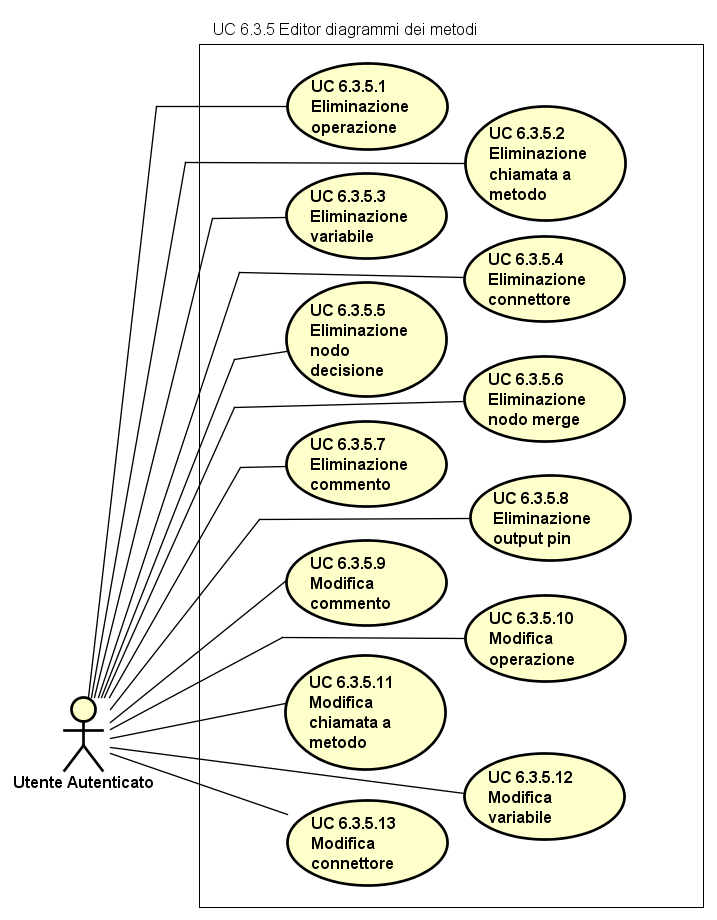
\includegraphics[scale=0.5]{../../Casi D'uso/UC6.3.5.png}
\caption{Caso d'uso UC6.3.5}
 \end{figure}
\begin{itemize}
\item \textbf{Attori}: \glossaryItem{Utente} autenticato;
\item \textbf{Descrizione}: L'attore può modificare il \glossaryItem{Diagramma} del \glossaryItem{Metodo} di una \glossaryItem{Classe};
\item \textbf{Precondizione}: Nell'\glossaryItem{Applicazione} è caricato correttamente un progetto che  contiene almeno una \glossaryItem{Classe} con un \glossaryItem{Metodo}, è visualizzata la finestra di modifica del \glossaryItem{Metodo};
\item \textbf{Postcondizione}: Il \glossaryItem{Diagramma} del \glossaryItem{Metodo} di una \glossaryItem{Classe} viene cambiato dalle eventuali modifiche dell'attore;
\item \textbf{Scenario principale}: \begin{enumerate}\item Eliminazione operazione (UC6.3.5.1);\item Modifica operazione (UC6.3.5.10);\item Modifica chiamata a \glossaryItem{Metodo} (UC6.3.5.11);\item Modifica variabile (UC6.3.5.12);\item Modifica connettore (UC6.3.5.13);\item Eliminazione chiamata a \glossaryItem{Metodo} (UC6.3.5.2);\item Eliminazione variabile (UC6.3.5.3);\item Eliminazione connettore (UC6.3.5.4);\item Eliminazione nodo decisione (UC6.3.5.5);\item Eliminazione nodo \glossaryItem{Merge} (UC6.3.5.6);\item Eliminazione commento (UC6.3.5.7);\item Eliminazione output pin (UC6.3.5.8);\item Modifica commento (UC6.3.5.9).
 \end{enumerate}
\end{itemize}
\subsection{UC6.3.5.1 - Eliminazione operazione}
\label{ssec:UC6.3.5.1}
\begin{itemize}
\item \textbf{Attori}: \glossaryItem{Utente} autenticato;
\item \textbf{Descrizione}: L'attore può eliminare un elemento operazione fra gli elementi del digramma del \glossaryItem{Metodo} di una \glossaryItem{Classe};
\item \textbf{Precondizione}: È visualizzato il \glossaryItem{Diagramma} di un \glossaryItem{Metodo} che contiene almeno un elemento operazione;
\item \textbf{Postcondizione}: Viene eliminato, dal \glossaryItem{Diagramma} del \glossaryItem{Metodo},  l'elemento operazione selezionato dall'attore;
\item \textbf{Scenario principale}: L'attore elimina un elemento operazione nel diagramma del metodo del codice.
\end{itemize}
\subsection{UC6.3.5.10 - Modifica operazione}
\label{ssec:UC6.3.5.10}
\begin{itemize}
\item \textbf{Attori}: \glossaryItem{Utente} autenticato;
\item \textbf{Descrizione}: L'attore ha la possibilità di modificare un elemento operazione presente nel \glossaryItem{Diagramma} del \glossaryItem{Metodo} di una \glossaryItem{Classe};
\item \textbf{Precondizione}: È visualizzato il \glossaryItem{Diagramma} di un \glossaryItem{Metodo} che contiene almeno un elemento operazione;
\item \textbf{Postcondizione}: Viene modificato l'elemento operazione con i cambiamenti apportati dall'\glossaryItem{Utente};
\item \textbf{Scenario principale}: \begin{enumerate}\item Definizione operazione (UC6.3.5.10.1).
 \end{enumerate}
\end{itemize}
\subsection{UC6.3.5.10.1 - Definizione operazione}
\label{ssec:UC6.3.5.10.1}
\begin{itemize}
\item \textbf{Attori}: \glossaryItem{Utente} autenticato;
\item \textbf{Descrizione}: L'attore ha la possibilità di definire un'operazione tramite input testuale;
\item \textbf{Precondizione}: È aperta la finestra di modifica di un elemento operazione;
\item \textbf{Postcondizione}: È applicata l'operazione definita dall'\glossaryItem{Utente};
\item \textbf{Scenario principale}: L'attore definisce un'operazione tramite input testuale nel diagramma del metodo del codice.
\end{itemize}
\subsection{UC6.3.5.11 - Modifica chiamata a metodo}
\label{ssec:UC6.3.5.11}
\begin{itemize}
\item \textbf{Attori}: \glossaryItem{Utente} autenticato;
\item \textbf{Descrizione}: L'attore può modificare l'elemento chiamata a \glossaryItem{Metodo} di un \glossaryItem{Diagramma} del \glossaryItem{Metodo} di una \glossaryItem{Classe};
\item \textbf{Precondizione}: È visualizzato il \glossaryItem{Diagramma} di un \glossaryItem{Metodo} che contiene almeno un elemento chiamata a \glossaryItem{Metodo};
\item \textbf{Postcondizione}: L'elemento chiamata a \glossaryItem{Metodo} viene modificato con le modifiche apportate dall'attore;
\item \textbf{Scenario principale}: \begin{enumerate}\item Selezione \glossaryItem{Metodo} (UC6.3.5.11.1).
 \end{enumerate}
\end{itemize}
\subsection{UC6.3.5.11.1 - Selezione metodo}
\label{ssec:UC6.3.5.11.1}
\begin{itemize}
\item \textbf{Attori}: \glossaryItem{Utente} autenticato;
\item \textbf{Descrizione}: L'attore può selezionare un \glossaryItem{Metodo} dalla lista dei \glossaryItem{Metodi}, e parametri in ingresso da esso richiesti;
\item \textbf{Precondizione}: La finestra di modifica di un elemento chiamata a \glossaryItem{Metodo} è visualizzata correttamente;
\item \textbf{Postcondizione}: Viene assegnato il \glossaryItem{Metodo}, selezionato dall'attore, all'elemento chiamata a \glossaryItem{Metodo} e eventuali parametri richiesti;
\item \textbf{Scenario principale}: L'attore seleziona un metodo della lista dei metodi del diagramma del metodo del codice.
\end{itemize}
\subsection{UC6.3.5.12 - Modifica variabile}
\label{ssec:UC6.3.5.12}
\begin{itemize}
\item \textbf{Attori}: \glossaryItem{Utente} autenticato;
\item \textbf{Descrizione}: L'attore può modificare l'elemento variabile di un \glossaryItem{Diagramma} del \glossaryItem{Metodo} di una \glossaryItem{Classe};
\item \textbf{Precondizione}: È visualizzato il \glossaryItem{Diagramma} di un \glossaryItem{Metodo} che contiene almeno un elemento variabile;
\item \textbf{Postcondizione}: L'elemento variabile viene modificato con le modifiche apportate dall'attore;
\item \textbf{Scenario principale}: \begin{enumerate}\item Istanziazione nuova variabile (UC6.3.5.12.1).
 \end{enumerate}
\end{itemize}
\subsection{UC6.3.5.12.1 - Istanziazione nuova variabile}
\label{ssec:UC6.3.5.12.1}
\begin{itemize}
\item \textbf{Attori}: \glossaryItem{Utente} autenticato;
\item \textbf{Descrizione}: L'attore può definire una nuova variabile per l'elemento variabile corrente;
\item \textbf{Precondizione}: Viene visualizzata correttamente la finestra di modifica dell'elemento variabile;
\item \textbf{Postcondizione}: È applicata, all'elemento variabile, la variabile definita dall'attore;
\item \textbf{Scenario principale}: L'attore istanzia una nuova variabile nel diagramma del metodo del codice.
\end{itemize}
\subsection{UC6.3.5.13 - Modifica connettore}
\label{ssec:UC6.3.5.13}
\begin{itemize}
\item \textbf{Attori}: \glossaryItem{Utente} autenticato;
\item \textbf{Descrizione}: L'attore può operare delle modifiche su un elemento connettore presente nel \glossaryItem{Diagramma} del \glossaryItem{Metodo} di una \glossaryItem{Classe};
\item \textbf{Precondizione}: È visualizzato il \glossaryItem{Diagramma} di un \glossaryItem{Metodo} che contiene almeno un elemento connettore;
\item \textbf{Postcondizione}: Vengono applicate le modifiche eventualmente apportate dall'attore;
\item \textbf{Scenario principale}: \begin{enumerate}\item Definizione condizione di guardia (UC6.3.5.13.1).
 \end{enumerate}
\end{itemize}
\subsection{UC6.3.5.13.1 - Definizione condizione di guardia}
\label{ssec:UC6.3.5.13.1}
\begin{itemize}
\item \textbf{Attori}: \glossaryItem{Utente} autenticato;
\item \textbf{Descrizione}: L'attore può definire una guardia per l'elemento connettore;
\item \textbf{Precondizione}: Viene visualizzata la finestra di modifica dell'elemento connettore;
\item \textbf{Postcondizione}: Viene ridefinita la guardia come specificato dall'attore;
\item \textbf{Scenario principale}: L'attore definisce una condizione di guardia per il connettore nel diagramma del metodo del codice.
\end{itemize}
\subsection{UC6.3.5.2 - Eliminazione chiamata a metodo}
\label{ssec:UC6.3.5.2}
\begin{itemize}
\item \textbf{Attori}: \glossaryItem{Utente} autenticato;
\item \textbf{Descrizione}: L'attore può eliminare, dal \glossaryItem{Diagramma} del \glossaryItem{Metodo} di una \glossaryItem{Classe}, un elemento chiamata a \glossaryItem{Metodo};
\item \textbf{Precondizione}: È visualizzato il \glossaryItem{Diagramma} di un \glossaryItem{Metodo} che contiene almeno un elemento chiamata a \glossaryItem{Metodo};
\item \textbf{Postcondizione}: Viene eliminato, dal \glossaryItem{Diagramma} del \glossaryItem{Metodo},  l'elemento chiamata a \glossaryItem{Metodo} selezionato dall'attore;
\item \textbf{Scenario principale}: L'attore elimina un elemento chiamata a metodo nel diagramma del metodo del codice.
\end{itemize}
\subsection{UC6.3.5.3 - Eliminazione variabile}
\label{ssec:UC6.3.5.3}
\begin{itemize}
\item \textbf{Attori}: \glossaryItem{Utente} autenticato;
\item \textbf{Descrizione}: L'attore può eliminare un elemento variabile presente nel \glossaryItem{Diagramma} del \glossaryItem{Metodo} di una \glossaryItem{Classe};
\item \textbf{Precondizione}: È visualizzato il \glossaryItem{Diagramma} di un \glossaryItem{Metodo} che contiene almeno un elemento variabile;
\item \textbf{Postcondizione}: Viene eliminato, dal \glossaryItem{Diagramma} del \glossaryItem{Metodo},  l'elemento variabile selezionato dall'attore;
\item \textbf{Scenario principale}: L'attore elimina un elemento variabile nel diagramma del metodo del codice.
\end{itemize}
\subsection{UC6.3.5.4 - Eliminazione connettore}
\label{ssec:UC6.3.5.4}
\begin{itemize}
\item \textbf{Attori}: \glossaryItem{Utente} autenticato;
\item \textbf{Descrizione}: L'attore può eliminare, dal \glossaryItem{Diagramma} del \glossaryItem{Metodo} di una \glossaryItem{Classe}, un elemento connettore;
\item \textbf{Precondizione}: È visualizzato il \glossaryItem{Diagramma} di un \glossaryItem{Metodo} che contiene almeno un elemento connettore;
\item \textbf{Postcondizione}: Viene eliminato, dal \glossaryItem{Diagramma} del \glossaryItem{Metodo},  l'elemento chiamata a \glossaryItem{Metodo} selezionato dall'attore;
\item \textbf{Scenario principale}: L'attore elimina un elemento connettore nel diagramma del metodo del codice.
\end{itemize}
\subsection{UC6.3.5.5 - Eliminazione nodo decisione}
\label{ssec:UC6.3.5.5}
\begin{itemize}
\item \textbf{Attori}: \glossaryItem{Utente} autenticato;
\item \textbf{Descrizione}: L'attore ha la possibilità di eliminare un elemento nodo decisione dal \glossaryItem{Diagramma} del \glossaryItem{Metodo} di una \glossaryItem{Classe};
\item \textbf{Precondizione}: È visualizzato il \glossaryItem{Diagramma} di un \glossaryItem{Metodo} che contiene almeno un elemento nodo decisione;
\item \textbf{Postcondizione}: Viene eliminato, dal \glossaryItem{Diagramma} del \glossaryItem{Metodo},  l'elemento nodo decisione selezionato dall'attore;
\item \textbf{Scenario principale}: L'attore elimina un elemento nodo di decisione nel diagramma del metodo del codice.
\end{itemize}
\subsection{UC6.3.5.6 - Eliminazione nodo merge}
\label{ssec:UC6.3.5.6}
\begin{itemize}
\item \textbf{Attori}: \glossaryItem{Utente} autenticato;
\item \textbf{Descrizione}: L'attore può eliminare, dal \glossaryItem{Diagramma} del \glossaryItem{Metodo} di una \glossaryItem{Classe}, un elemento nodo \glossaryItem{Merge};
\item \textbf{Precondizione}: È visualizzato il \glossaryItem{Diagramma} di un \glossaryItem{Metodo} che contiene almeno un elemento nodo \glossaryItem{Merge};
\item \textbf{Postcondizione}: Viene eliminato, dal \glossaryItem{Diagramma} del \glossaryItem{Metodo},  l'elemento nodo \glossaryItem{Merge} selezionato dall'attore;
\item \textbf{Scenario principale}: L'attore elimina un elemento nodo merge nel diagramma del metodo del codice.
\end{itemize}
\subsection{UC6.3.5.7 - Eliminazione commento}
\label{ssec:UC6.3.5.7}
\begin{itemize}
\item \textbf{Attori}: \glossaryItem{Utente} autenticato;
\item \textbf{Descrizione}: L'attore può eliminare, dal \glossaryItem{Diagramma} del \glossaryItem{Metodo} di una \glossaryItem{Classe}, un elemento commento;
\item \textbf{Precondizione}: È visualizzato il \glossaryItem{Diagramma} di un \glossaryItem{Metodo} che contiene almeno un elemento commento;
\item \textbf{Postcondizione}: Viene eliminato, dal \glossaryItem{Diagramma} del \glossaryItem{Metodo},  l'elemento commento selezionato dall'attore;
\item \textbf{Scenario principale}: L'attore elimina un elemento commento nel diagramma del metodo del codice.
\end{itemize}
\subsection{UC6.3.5.8 - Eliminazione output pin}
\label{ssec:UC6.3.5.8}
\begin{itemize}
\item \textbf{Attori}: \glossaryItem{Utente} autenticato;
\item \textbf{Descrizione}: L'attore può eliminare, dal \glossaryItem{Diagramma} del \glossaryItem{Metodo} di una \glossaryItem{Classe}, un elemento output pin;
\item \textbf{Precondizione}: È visualizzato il \glossaryItem{Diagramma} di un \glossaryItem{Metodo} che contiene almeno un elemento output pin;
\item \textbf{Postcondizione}: L'elemento output pin, selezionato dall'\glossaryItem{Utente}, viene rimosso dal \glossaryItem{Diagramma} del \glossaryItem{Metodo};
\item \textbf{Scenario principale}: L'attore elimina un elemento output pin nel diagramma del metodo del codice.
\end{itemize}
\subsection{UC6.3.5.9 - Modifica commento}
\label{ssec:UC6.3.5.9}
\begin{itemize}
\item \textbf{Attori}: \glossaryItem{Utente} autenticato;
\item \textbf{Descrizione}: L'attore può modificare un elemento commento presente nel \glossaryItem{Diagramma} del \glossaryItem{Metodo} di una \glossaryItem{Classe};
\item \textbf{Precondizione}: È visualizzato il \glossaryItem{Diagramma} di un \glossaryItem{Metodo} che contiene almeno un elemento commento;
\item \textbf{Postcondizione}: Vengono apportate le modifiche, all'elemento commento, effettuate dall'attore.
\item \textbf{Scenario principale}: L'attore modifica un elemento commento nel diagramma del metodo del codice.
\end{itemize};
\newpage
\subsection{UC6.4 - Pannello laterale}
\label{ssec:UC6.4}

\begin{figure}[h!]
\centering
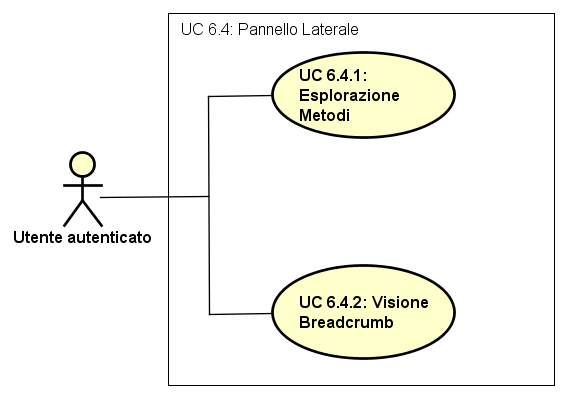
\includegraphics[scale=0.5]{../../Casi D'uso/UC6.4.png}
\caption{Caso d'uso UC6.4}
 \end{figure}
\begin{itemize}
\item \textbf{Attori}: \glossaryItem{Utente} autenticato;
\item \textbf{Descrizione}: L'attore può accedere a questa sezione di schermo nella quale è possibile visionare il flusso del programma a partire dal \glossaryItem{Metodo} main;
\item \textbf{Precondizione}: È aperto un progetto;
\item \textbf{Postcondizione}: Visualizza un \glossaryItem{Diagramma delle attività};
\item \textbf{Scenario principale}: \begin{enumerate}\item Esplorazione \glossaryItem{Metodi} (UC6.4.1);\item Visione Breadcrumb (UC6.4.2).
 \end{enumerate}
\end{itemize}
\subsection{UC6.4.1 - Esplorazione metodi}
\label{ssec:UC6.4.1}
\begin{itemize}
\item \textbf{Attori}: \glossaryItem{Utente} autenticato;
\item \textbf{Descrizione}: L'attore, selezionando una chiamata a \glossaryItem{Metodo}, può visionare il \glossaryItem{Diagramma delle attività} di tale \glossaryItem{Metodo};
\item \textbf{Precondizione}: È visualizzato un \glossaryItem{Diagramma delle attività};
\item \textbf{Postcondizione}: Viene mostrato il \glossaryItem{Diagramma delle attività} del \glossaryItem{Metodo} selezionato;
\item \textbf{Scenario principale}: L'attore seleziona un elemento "chiamata a metodo" per visionare il diagramma delle attività di tale metodo.
\end{itemize}
\subsection{UC6.4.2 - Visione Breadcrumb}
\label{ssec:UC6.4.2}
\begin{itemize}
\item \textbf{Attori}: \glossaryItem{Utente} autenticato;
\item \textbf{Descrizione}: Viene visualizzata una Breadcrumb che rappresenta il percorso effettuato dall'\glossaryItem{Utente} durante la navigazione dei vari \glossaryItem{Metodo} selezionati;
\item \textbf{Precondizione}: E' visualizzato un \glossaryItem{Diagramma delle attività};
\item \textbf{Postcondizione}: Vengono visualizzati in ordine di accesso tutti i \glossaryItem{Metodi} selezionati dall'\glossaryItem{Utente} nella visione principale del programma;
\item \textbf{Scenario principale}: L'attore visiona i vari metodi selezionati durante la navigazione tra le chiamate a metodi.
\end{itemize}
